\documentclass[11pt]{article}
    \usepackage[slantfont, boldfont]{xeCJK}
    \setCJKmainfont{Sarasa UI SC}
    \usepackage[breakable]{tcolorbox}
    \usepackage{parskip} % Stop auto-indenting (to mimic markdown behaviour)
    
    \usepackage{iftex}
    \ifPDFTeX
    	\usepackage[T1]{fontenc}
    	\usepackage{mathpazo}
    \else
    	\usepackage{fontspec}
    \fi

    % Basic figure setup, for now with no caption control since it's done
    % automatically by Pandoc (which extracts ![](path) syntax from Markdown).
    \usepackage{graphicx}
    % Maintain compatibility with old templates. Remove in nbconvert 6.0
    \let\Oldincludegraphics\includegraphics
    % Ensure that by default, figures have no caption (until we provide a
    % proper Figure object with a Caption API and a way to capture that
    % in the conversion process - todo).
    \usepackage{caption}
    \DeclareCaptionFormat{nocaption}{}
    \captionsetup{format=nocaption,aboveskip=0pt,belowskip=0pt}

    \usepackage{float}
    \floatplacement{figure}{H} % forces figures to be placed at the correct location
    \usepackage{xcolor} % Allow colors to be defined
    \usepackage{enumerate} % Needed for markdown enumerations to work
    \usepackage{geometry} % Used to adjust the document margins
    \usepackage{amsmath} % Equations
    \usepackage{amssymb} % Equations
    \usepackage{textcomp} % defines textquotesingle
    % Hack from http://tex.stackexchange.com/a/47451/13684:
    \AtBeginDocument{%
        \def\PYZsq{\textquotesingle}% Upright quotes in Pygmentized code
    }
    \usepackage{upquote} % Upright quotes for verbatim code
    \usepackage{eurosym} % defines \euro
    \usepackage[mathletters]{ucs} % Extended unicode (utf-8) support
    \usepackage{fancyvrb} % verbatim replacement that allows latex
    \usepackage{grffile} % extends the file name processing of package graphics 
                         % to support a larger range
    \makeatletter % fix for old versions of grffile with XeLaTeX
    \@ifpackagelater{grffile}{2019/11/01}
    {
      % Do nothing on new versions
    }
    {
      \def\Gread@@xetex#1{%
        \IfFileExists{"\Gin@base".bb}%
        {\Gread@eps{\Gin@base.bb}}%
        {\Gread@@xetex@aux#1}%
      }
    }
    \makeatother
    \usepackage[Export]{adjustbox} % Used to constrain images to a maximum size
    \adjustboxset{max size={0.9\linewidth}{0.9\paperheight}}

    % The hyperref package gives us a pdf with properly built
    % internal navigation ('pdf bookmarks' for the table of contents,
    % internal cross-reference links, web links for URLs, etc.)
    \usepackage{hyperref}
    % The default LaTeX title has an obnoxious amount of whitespace. By default,
    % titling removes some of it. It also provides customization options.
    \usepackage{titling}
    \usepackage{longtable} % longtable support required by pandoc >1.10
    \usepackage{booktabs}  % table support for pandoc > 1.12.2
    \usepackage[inline]{enumitem} % IRkernel/repr support (it uses the enumerate* environment)
    \usepackage[normalem]{ulem} % ulem is needed to support strikethroughs (\sout)
                                % normalem makes italics be italics, not underlines
    \usepackage{mathrsfs}
    

    
    % Colors for the hyperref package
    \definecolor{urlcolor}{rgb}{0,.145,.698}
    \definecolor{linkcolor}{rgb}{.71,0.21,0.01}
    \definecolor{citecolor}{rgb}{.12,.54,.11}

    % ANSI colors
    \definecolor{ansi-black}{HTML}{3E424D}
    \definecolor{ansi-black-intense}{HTML}{282C36}
    \definecolor{ansi-red}{HTML}{E75C58}
    \definecolor{ansi-red-intense}{HTML}{B22B31}
    \definecolor{ansi-green}{HTML}{00A250}
    \definecolor{ansi-green-intense}{HTML}{007427}
    \definecolor{ansi-yellow}{HTML}{DDB62B}
    \definecolor{ansi-yellow-intense}{HTML}{B27D12}
    \definecolor{ansi-blue}{HTML}{208FFB}
    \definecolor{ansi-blue-intense}{HTML}{0065CA}
    \definecolor{ansi-magenta}{HTML}{D160C4}
    \definecolor{ansi-magenta-intense}{HTML}{A03196}
    \definecolor{ansi-cyan}{HTML}{60C6C8}
    \definecolor{ansi-cyan-intense}{HTML}{258F8F}
    \definecolor{ansi-white}{HTML}{C5C1B4}
    \definecolor{ansi-white-intense}{HTML}{A1A6B2}
    \definecolor{ansi-default-inverse-fg}{HTML}{FFFFFF}
    \definecolor{ansi-default-inverse-bg}{HTML}{000000}

    % common color for the border for error outputs.
    \definecolor{outerrorbackground}{HTML}{FFDFDF}

    % commands and environments needed by pandoc snippets
    % extracted from the output of `pandoc -s`
    \providecommand{\tightlist}{%
      \setlength{\itemsep}{0pt}\setlength{\parskip}{0pt}}
    \DefineVerbatimEnvironment{Highlighting}{Verbatim}{commandchars=\\\{\}}
    % Add ',fontsize=\small' for more characters per line
    \newenvironment{Shaded}{}{}
    \newcommand{\KeywordTok}[1]{\textcolor[rgb]{0.00,0.44,0.13}{\textbf{{#1}}}}
    \newcommand{\DataTypeTok}[1]{\textcolor[rgb]{0.56,0.13,0.00}{{#1}}}
    \newcommand{\DecValTok}[1]{\textcolor[rgb]{0.25,0.63,0.44}{{#1}}}
    \newcommand{\BaseNTok}[1]{\textcolor[rgb]{0.25,0.63,0.44}{{#1}}}
    \newcommand{\FloatTok}[1]{\textcolor[rgb]{0.25,0.63,0.44}{{#1}}}
    \newcommand{\CharTok}[1]{\textcolor[rgb]{0.25,0.44,0.63}{{#1}}}
    \newcommand{\StringTok}[1]{\textcolor[rgb]{0.25,0.44,0.63}{{#1}}}
    \newcommand{\CommentTok}[1]{\textcolor[rgb]{0.38,0.63,0.69}{\textit{{#1}}}}
    \newcommand{\OtherTok}[1]{\textcolor[rgb]{0.00,0.44,0.13}{{#1}}}
    \newcommand{\AlertTok}[1]{\textcolor[rgb]{1.00,0.00,0.00}{\textbf{{#1}}}}
    \newcommand{\FunctionTok}[1]{\textcolor[rgb]{0.02,0.16,0.49}{{#1}}}
    \newcommand{\RegionMarkerTok}[1]{{#1}}
    \newcommand{\ErrorTok}[1]{\textcolor[rgb]{1.00,0.00,0.00}{\textbf{{#1}}}}
    \newcommand{\NormalTok}[1]{{#1}}
    
    % Additional commands for more recent versions of Pandoc
    \newcommand{\ConstantTok}[1]{\textcolor[rgb]{0.53,0.00,0.00}{{#1}}}
    \newcommand{\SpecialCharTok}[1]{\textcolor[rgb]{0.25,0.44,0.63}{{#1}}}
    \newcommand{\VerbatimStringTok}[1]{\textcolor[rgb]{0.25,0.44,0.63}{{#1}}}
    \newcommand{\SpecialStringTok}[1]{\textcolor[rgb]{0.73,0.40,0.53}{{#1}}}
    \newcommand{\ImportTok}[1]{{#1}}
    \newcommand{\DocumentationTok}[1]{\textcolor[rgb]{0.73,0.13,0.13}{\textit{{#1}}}}
    \newcommand{\AnnotationTok}[1]{\textcolor[rgb]{0.38,0.63,0.69}{\textbf{\textit{{#1}}}}}
    \newcommand{\CommentVarTok}[1]{\textcolor[rgb]{0.38,0.63,0.69}{\textbf{\textit{{#1}}}}}
    \newcommand{\VariableTok}[1]{\textcolor[rgb]{0.10,0.09,0.49}{{#1}}}
    \newcommand{\ControlFlowTok}[1]{\textcolor[rgb]{0.00,0.44,0.13}{\textbf{{#1}}}}
    \newcommand{\OperatorTok}[1]{\textcolor[rgb]{0.40,0.40,0.40}{{#1}}}
    \newcommand{\BuiltInTok}[1]{{#1}}
    \newcommand{\ExtensionTok}[1]{{#1}}
    \newcommand{\PreprocessorTok}[1]{\textcolor[rgb]{0.74,0.48,0.00}{{#1}}}
    \newcommand{\AttributeTok}[1]{\textcolor[rgb]{0.49,0.56,0.16}{{#1}}}
    \newcommand{\InformationTok}[1]{\textcolor[rgb]{0.38,0.63,0.69}{\textbf{\textit{{#1}}}}}
    \newcommand{\WarningTok}[1]{\textcolor[rgb]{0.38,0.63,0.69}{\textbf{\textit{{#1}}}}}
    
    
    % Define a nice break command that doesn't care if a line doesn't already
    % exist.
    \def\br{\hspace*{\fill} \\* }
    % Math Jax compatibility definitions
    \def\gt{>}
    \def\lt{<}
    \let\Oldtex\TeX
    \let\Oldlatex\LaTeX
    \renewcommand{\TeX}{\textrm{\Oldtex}}
    \renewcommand{\LaTeX}{\textrm{\Oldlatex}}
    % Document parameters
    % Document title
    \title{黄师姐 Python 秘籍}
    
    
    
    
    
% Pygments definitions
\makeatletter
\def\PY@reset{\let\PY@it=\relax \let\PY@bf=\relax%
    \let\PY@ul=\relax \let\PY@tc=\relax%
    \let\PY@bc=\relax \let\PY@ff=\relax}
\def\PY@tok#1{\csname PY@tok@#1\endcsname}
\def\PY@toks#1+{\ifx\relax#1\empty\else%
    \PY@tok{#1}\expandafter\PY@toks\fi}
\def\PY@do#1{\PY@bc{\PY@tc{\PY@ul{%
    \PY@it{\PY@bf{\PY@ff{#1}}}}}}}
\def\PY#1#2{\PY@reset\PY@toks#1+\relax+\PY@do{#2}}

\@namedef{PY@tok@w}{\def\PY@tc##1{\textcolor[rgb]{0.73,0.73,0.73}{##1}}}
\@namedef{PY@tok@c}{\let\PY@it=\textit\def\PY@tc##1{\textcolor[rgb]{0.25,0.50,0.50}{##1}}}
\@namedef{PY@tok@cp}{\def\PY@tc##1{\textcolor[rgb]{0.74,0.48,0.00}{##1}}}
\@namedef{PY@tok@k}{\let\PY@bf=\textbf\def\PY@tc##1{\textcolor[rgb]{0.00,0.50,0.00}{##1}}}
\@namedef{PY@tok@kp}{\def\PY@tc##1{\textcolor[rgb]{0.00,0.50,0.00}{##1}}}
\@namedef{PY@tok@kt}{\def\PY@tc##1{\textcolor[rgb]{0.69,0.00,0.25}{##1}}}
\@namedef{PY@tok@o}{\def\PY@tc##1{\textcolor[rgb]{0.40,0.40,0.40}{##1}}}
\@namedef{PY@tok@ow}{\let\PY@bf=\textbf\def\PY@tc##1{\textcolor[rgb]{0.67,0.13,1.00}{##1}}}
\@namedef{PY@tok@nb}{\def\PY@tc##1{\textcolor[rgb]{0.00,0.50,0.00}{##1}}}
\@namedef{PY@tok@nf}{\def\PY@tc##1{\textcolor[rgb]{0.00,0.00,1.00}{##1}}}
\@namedef{PY@tok@nc}{\let\PY@bf=\textbf\def\PY@tc##1{\textcolor[rgb]{0.00,0.00,1.00}{##1}}}
\@namedef{PY@tok@nn}{\let\PY@bf=\textbf\def\PY@tc##1{\textcolor[rgb]{0.00,0.00,1.00}{##1}}}
\@namedef{PY@tok@ne}{\let\PY@bf=\textbf\def\PY@tc##1{\textcolor[rgb]{0.82,0.25,0.23}{##1}}}
\@namedef{PY@tok@nv}{\def\PY@tc##1{\textcolor[rgb]{0.10,0.09,0.49}{##1}}}
\@namedef{PY@tok@no}{\def\PY@tc##1{\textcolor[rgb]{0.53,0.00,0.00}{##1}}}
\@namedef{PY@tok@nl}{\def\PY@tc##1{\textcolor[rgb]{0.63,0.63,0.00}{##1}}}
\@namedef{PY@tok@ni}{\let\PY@bf=\textbf\def\PY@tc##1{\textcolor[rgb]{0.60,0.60,0.60}{##1}}}
\@namedef{PY@tok@na}{\def\PY@tc##1{\textcolor[rgb]{0.49,0.56,0.16}{##1}}}
\@namedef{PY@tok@nt}{\let\PY@bf=\textbf\def\PY@tc##1{\textcolor[rgb]{0.00,0.50,0.00}{##1}}}
\@namedef{PY@tok@nd}{\def\PY@tc##1{\textcolor[rgb]{0.67,0.13,1.00}{##1}}}
\@namedef{PY@tok@s}{\def\PY@tc##1{\textcolor[rgb]{0.73,0.13,0.13}{##1}}}
\@namedef{PY@tok@sd}{\let\PY@it=\textit\def\PY@tc##1{\textcolor[rgb]{0.73,0.13,0.13}{##1}}}
\@namedef{PY@tok@si}{\let\PY@bf=\textbf\def\PY@tc##1{\textcolor[rgb]{0.73,0.40,0.53}{##1}}}
\@namedef{PY@tok@se}{\let\PY@bf=\textbf\def\PY@tc##1{\textcolor[rgb]{0.73,0.40,0.13}{##1}}}
\@namedef{PY@tok@sr}{\def\PY@tc##1{\textcolor[rgb]{0.73,0.40,0.53}{##1}}}
\@namedef{PY@tok@ss}{\def\PY@tc##1{\textcolor[rgb]{0.10,0.09,0.49}{##1}}}
\@namedef{PY@tok@sx}{\def\PY@tc##1{\textcolor[rgb]{0.00,0.50,0.00}{##1}}}
\@namedef{PY@tok@m}{\def\PY@tc##1{\textcolor[rgb]{0.40,0.40,0.40}{##1}}}
\@namedef{PY@tok@gh}{\let\PY@bf=\textbf\def\PY@tc##1{\textcolor[rgb]{0.00,0.00,0.50}{##1}}}
\@namedef{PY@tok@gu}{\let\PY@bf=\textbf\def\PY@tc##1{\textcolor[rgb]{0.50,0.00,0.50}{##1}}}
\@namedef{PY@tok@gd}{\def\PY@tc##1{\textcolor[rgb]{0.63,0.00,0.00}{##1}}}
\@namedef{PY@tok@gi}{\def\PY@tc##1{\textcolor[rgb]{0.00,0.63,0.00}{##1}}}
\@namedef{PY@tok@gr}{\def\PY@tc##1{\textcolor[rgb]{1.00,0.00,0.00}{##1}}}
\@namedef{PY@tok@ge}{\let\PY@it=\textit}
\@namedef{PY@tok@gs}{\let\PY@bf=\textbf}
\@namedef{PY@tok@gp}{\let\PY@bf=\textbf\def\PY@tc##1{\textcolor[rgb]{0.00,0.00,0.50}{##1}}}
\@namedef{PY@tok@go}{\def\PY@tc##1{\textcolor[rgb]{0.53,0.53,0.53}{##1}}}
\@namedef{PY@tok@gt}{\def\PY@tc##1{\textcolor[rgb]{0.00,0.27,0.87}{##1}}}
\@namedef{PY@tok@err}{\def\PY@bc##1{{\setlength{\fboxsep}{\string -\fboxrule}\fcolorbox[rgb]{1.00,0.00,0.00}{1,1,1}{\strut ##1}}}}
\@namedef{PY@tok@kc}{\let\PY@bf=\textbf\def\PY@tc##1{\textcolor[rgb]{0.00,0.50,0.00}{##1}}}
\@namedef{PY@tok@kd}{\let\PY@bf=\textbf\def\PY@tc##1{\textcolor[rgb]{0.00,0.50,0.00}{##1}}}
\@namedef{PY@tok@kn}{\let\PY@bf=\textbf\def\PY@tc##1{\textcolor[rgb]{0.00,0.50,0.00}{##1}}}
\@namedef{PY@tok@kr}{\let\PY@bf=\textbf\def\PY@tc##1{\textcolor[rgb]{0.00,0.50,0.00}{##1}}}
\@namedef{PY@tok@bp}{\def\PY@tc##1{\textcolor[rgb]{0.00,0.50,0.00}{##1}}}
\@namedef{PY@tok@fm}{\def\PY@tc##1{\textcolor[rgb]{0.00,0.00,1.00}{##1}}}
\@namedef{PY@tok@vc}{\def\PY@tc##1{\textcolor[rgb]{0.10,0.09,0.49}{##1}}}
\@namedef{PY@tok@vg}{\def\PY@tc##1{\textcolor[rgb]{0.10,0.09,0.49}{##1}}}
\@namedef{PY@tok@vi}{\def\PY@tc##1{\textcolor[rgb]{0.10,0.09,0.49}{##1}}}
\@namedef{PY@tok@vm}{\def\PY@tc##1{\textcolor[rgb]{0.10,0.09,0.49}{##1}}}
\@namedef{PY@tok@sa}{\def\PY@tc##1{\textcolor[rgb]{0.73,0.13,0.13}{##1}}}
\@namedef{PY@tok@sb}{\def\PY@tc##1{\textcolor[rgb]{0.73,0.13,0.13}{##1}}}
\@namedef{PY@tok@sc}{\def\PY@tc##1{\textcolor[rgb]{0.73,0.13,0.13}{##1}}}
\@namedef{PY@tok@dl}{\def\PY@tc##1{\textcolor[rgb]{0.73,0.13,0.13}{##1}}}
\@namedef{PY@tok@s2}{\def\PY@tc##1{\textcolor[rgb]{0.73,0.13,0.13}{##1}}}
\@namedef{PY@tok@sh}{\def\PY@tc##1{\textcolor[rgb]{0.73,0.13,0.13}{##1}}}
\@namedef{PY@tok@s1}{\def\PY@tc##1{\textcolor[rgb]{0.73,0.13,0.13}{##1}}}
\@namedef{PY@tok@mb}{\def\PY@tc##1{\textcolor[rgb]{0.40,0.40,0.40}{##1}}}
\@namedef{PY@tok@mf}{\def\PY@tc##1{\textcolor[rgb]{0.40,0.40,0.40}{##1}}}
\@namedef{PY@tok@mh}{\def\PY@tc##1{\textcolor[rgb]{0.40,0.40,0.40}{##1}}}
\@namedef{PY@tok@mi}{\def\PY@tc##1{\textcolor[rgb]{0.40,0.40,0.40}{##1}}}
\@namedef{PY@tok@il}{\def\PY@tc##1{\textcolor[rgb]{0.40,0.40,0.40}{##1}}}
\@namedef{PY@tok@mo}{\def\PY@tc##1{\textcolor[rgb]{0.40,0.40,0.40}{##1}}}
\@namedef{PY@tok@ch}{\let\PY@it=\textit\def\PY@tc##1{\textcolor[rgb]{0.25,0.50,0.50}{##1}}}
\@namedef{PY@tok@cm}{\let\PY@it=\textit\def\PY@tc##1{\textcolor[rgb]{0.25,0.50,0.50}{##1}}}
\@namedef{PY@tok@cpf}{\let\PY@it=\textit\def\PY@tc##1{\textcolor[rgb]{0.25,0.50,0.50}{##1}}}
\@namedef{PY@tok@c1}{\let\PY@it=\textit\def\PY@tc##1{\textcolor[rgb]{0.25,0.50,0.50}{##1}}}
\@namedef{PY@tok@cs}{\let\PY@it=\textit\def\PY@tc##1{\textcolor[rgb]{0.25,0.50,0.50}{##1}}}

\def\PYZbs{\char`\\}
\def\PYZus{\char`\_}
\def\PYZob{\char`\{}
\def\PYZcb{\char`\}}
\def\PYZca{\char`\^}
\def\PYZam{\char`\&}
\def\PYZlt{\char`\<}
\def\PYZgt{\char`\>}
\def\PYZsh{\char`\#}
\def\PYZpc{\char`\%}
\def\PYZdl{\char`\$}
\def\PYZhy{\char`\-}
\def\PYZsq{\char`\'}
\def\PYZdq{\char`\"}
\def\PYZti{\char`\~}
% for compatibility with earlier versions
\def\PYZat{@}
\def\PYZlb{[}
\def\PYZrb{]}
\makeatother


    % For linebreaks inside Verbatim environment from package fancyvrb. 
    \makeatletter
        \newbox\Wrappedcontinuationbox 
        \newbox\Wrappedvisiblespacebox 
        \newcommand*\Wrappedvisiblespace {\textcolor{red}{\textvisiblespace}} 
        \newcommand*\Wrappedcontinuationsymbol {\textcolor{red}{\llap{\tiny$\m@th\hookrightarrow$}}} 
        \newcommand*\Wrappedcontinuationindent {3ex } 
        \newcommand*\Wrappedafterbreak {\kern\Wrappedcontinuationindent\copy\Wrappedcontinuationbox} 
        % Take advantage of the already applied Pygments mark-up to insert 
        % potential linebreaks for TeX processing. 
        %        {, <, #, %, $, ' and ": go to next line. 
        %        _, }, ^, &, >, - and ~: stay at end of broken line. 
        % Use of \textquotesingle for straight quote. 
        \newcommand*\Wrappedbreaksatspecials {% 
            \def\PYGZus{\discretionary{\char`\_}{\Wrappedafterbreak}{\char`\_}}% 
            \def\PYGZob{\discretionary{}{\Wrappedafterbreak\char`\{}{\char`\{}}% 
            \def\PYGZcb{\discretionary{\char`\}}{\Wrappedafterbreak}{\char`\}}}% 
            \def\PYGZca{\discretionary{\char`\^}{\Wrappedafterbreak}{\char`\^}}% 
            \def\PYGZam{\discretionary{\char`\&}{\Wrappedafterbreak}{\char`\&}}% 
            \def\PYGZlt{\discretionary{}{\Wrappedafterbreak\char`\<}{\char`\<}}% 
            \def\PYGZgt{\discretionary{\char`\>}{\Wrappedafterbreak}{\char`\>}}% 
            \def\PYGZsh{\discretionary{}{\Wrappedafterbreak\char`\#}{\char`\#}}% 
            \def\PYGZpc{\discretionary{}{\Wrappedafterbreak\char`\%}{\char`\%}}% 
            \def\PYGZdl{\discretionary{}{\Wrappedafterbreak\char`\$}{\char`\$}}% 
            \def\PYGZhy{\discretionary{\char`\-}{\Wrappedafterbreak}{\char`\-}}% 
            \def\PYGZsq{\discretionary{}{\Wrappedafterbreak\textquotesingle}{\textquotesingle}}% 
            \def\PYGZdq{\discretionary{}{\Wrappedafterbreak\char`\"}{\char`\"}}% 
            \def\PYGZti{\discretionary{\char`\~}{\Wrappedafterbreak}{\char`\~}}% 
        } 
        % Some characters . , ; ? ! / are not pygmentized. 
        % This macro makes them "active" and they will insert potential linebreaks 
        \newcommand*\Wrappedbreaksatpunct {% 
            \lccode`\~`\.\lowercase{\def~}{\discretionary{\hbox{\char`\.}}{\Wrappedafterbreak}{\hbox{\char`\.}}}% 
            \lccode`\~`\,\lowercase{\def~}{\discretionary{\hbox{\char`\,}}{\Wrappedafterbreak}{\hbox{\char`\,}}}% 
            \lccode`\~`\;\lowercase{\def~}{\discretionary{\hbox{\char`\;}}{\Wrappedafterbreak}{\hbox{\char`\;}}}% 
            \lccode`\~`\:\lowercase{\def~}{\discretionary{\hbox{\char`\:}}{\Wrappedafterbreak}{\hbox{\char`\:}}}% 
            \lccode`\~`\?\lowercase{\def~}{\discretionary{\hbox{\char`\?}}{\Wrappedafterbreak}{\hbox{\char`\?}}}% 
            \lccode`\~`\!\lowercase{\def~}{\discretionary{\hbox{\char`\!}}{\Wrappedafterbreak}{\hbox{\char`\!}}}% 
            \lccode`\~`\/\lowercase{\def~}{\discretionary{\hbox{\char`\/}}{\Wrappedafterbreak}{\hbox{\char`\/}}}% 
            \catcode`\.\active
            \catcode`\,\active 
            \catcode`\;\active
            \catcode`\:\active
            \catcode`\?\active
            \catcode`\!\active
            \catcode`\/\active 
            \lccode`\~`\~ 	
        }
    \makeatother

    \let\OriginalVerbatim=\Verbatim
    \makeatletter
    \renewcommand{\Verbatim}[1][1]{%
        %\parskip\z@skip
        \sbox\Wrappedcontinuationbox {\Wrappedcontinuationsymbol}%
        \sbox\Wrappedvisiblespacebox {\FV@SetupFont\Wrappedvisiblespace}%
        \def\FancyVerbFormatLine ##1{\hsize\linewidth
            \vtop{\raggedright\hyphenpenalty\z@\exhyphenpenalty\z@
                \doublehyphendemerits\z@\finalhyphendemerits\z@
                \strut ##1\strut}%
        }%
        % If the linebreak is at a space, the latter will be displayed as visible
        % space at end of first line, and a continuation symbol starts next line.
        % Stretch/shrink are however usually zero for typewriter font.
        \def\FV@Space {%
            \nobreak\hskip\z@ plus\fontdimen3\font minus\fontdimen4\font
            \discretionary{\copy\Wrappedvisiblespacebox}{\Wrappedafterbreak}
            {\kern\fontdimen2\font}%
        }%
        
        % Allow breaks at special characters using \PYG... macros.
        \Wrappedbreaksatspecials
        % Breaks at punctuation characters . , ; ? ! and / need catcode=\active 	
        \OriginalVerbatim[#1,codes*=\Wrappedbreaksatpunct]%
    }
    \makeatother

    % Exact colors from NB
    \definecolor{incolor}{HTML}{303F9F}
    \definecolor{outcolor}{HTML}{D84315}
    \definecolor{cellborder}{HTML}{CFCFCF}
    \definecolor{cellbackground}{HTML}{F7F7F7}
    
    % prompt
    \makeatletter
    \newcommand{\boxspacing}{\kern\kvtcb@left@rule\kern\kvtcb@boxsep}
    \makeatother
    \newcommand{\prompt}[4]{
        {\ttfamily\llap{{\color{#2}[#3]:\hspace{3pt}#4}}\vspace{-\baselineskip}}
    }
    

    
    % Prevent overflowing lines due to hard-to-break entities
    \sloppy 
    % Setup hyperref package
    \hypersetup{
      breaklinks=true,  % so long urls are correctly broken across lines
      colorlinks=true,
      urlcolor=urlcolor,
      linkcolor=linkcolor,
      citecolor=citecolor,
      }
    % Slightly bigger margins than the latex defaults
    
    \geometry{verbose,tmargin=1in,bmargin=1in,lmargin=1in,rmargin=1in}
    
    

\begin{document}
    
    \maketitle
    
    

    
    \hypertarget{python-ux590dux4e60ux77e5ux8bc6ux70b9}{%
\section{Python
复习知识点}\label{python-ux590dux4e60ux77e5ux8bc6ux70b9}}

\hypertarget{ux77e5ux8bc6ux70b9}{%
\subsection{知识点}\label{ux77e5ux8bc6ux70b9}}

\begin{itemize}
\tightlist
\item
  1. Python程序需要\textbf{描述数据}和\textbf{操作数据}。
\item
  2. Python程序区分大小写
\item
  3. 标识符的基本要求 - 驼峰法则(\texttt{camelCase}) /
  匈牙利法则(\texttt{Hungarian\ notation})

  \begin{itemize}
  \tightlist
  \item
    \texttt{iPhone}
  \item
    \texttt{eBay}
  \item
    \texttt{johnSmith}
  \end{itemize}
\item
  4. 变量赋值及相应的类型(主要的基本数据类型)
\end{itemize}

    \begin{longtable}[]{@{}ll@{}}
\toprule
类型 & 典型值 \\
\midrule
\endhead
布尔型(bool) & \texttt{True}, \texttt{False} \\
整形(int) & \texttt{1}, \texttt{100} \\
浮点型(float) & \texttt{3.1415926} \\
复数(complex) & \texttt{1+2j} \\
字符串(string) & \texttt{\textquotesingle{}hello\textquotesingle{}} \\
\bottomrule
\end{longtable}

    \begin{itemize}
\tightlist
\item
  5. 注意\texttt{=}与\texttt{==}的区别

  \begin{itemize}
  \tightlist
  \item
    赋值运算符(\texttt{=}) - \texttt{a\ =\ 10}
    把\texttt{10}赋给变量\texttt{a}。
  \item
    比较运算符(\texttt{==}) - \texttt{a\ ==\ 10}
    比较\texttt{a}和\texttt{10}是否相等,相等返回\texttt{True},不相等返回\texttt{False}。
  \end{itemize}
\item
  6. 特殊字符换行符\texttt{\textbackslash{}n}
\end{itemize}

    \begin{tcolorbox}[breakable, size=fbox, boxrule=1pt, pad at break*=1mm,colback=cellbackground, colframe=cellborder]
\prompt{In}{incolor}{1}{\boxspacing}
\begin{Verbatim}[commandchars=\\\{\}]
\PY{n+nb}{print}\PY{p}{(}\PY{l+s+s2}{\PYZdq{}}\PY{l+s+s2}{hello}\PY{l+s+se}{\PYZbs{}n}\PY{l+s+s2}{world}\PY{l+s+s2}{\PYZdq{}}\PY{p}{)}
\end{Verbatim}
\end{tcolorbox}

    \begin{Verbatim}[commandchars=\\\{\}]
hello
world
    \end{Verbatim}

    \begin{tcolorbox}[breakable, size=fbox, boxrule=1pt, pad at break*=1mm,colback=cellbackground, colframe=cellborder]
\prompt{In}{incolor}{2}{\boxspacing}
\begin{Verbatim}[commandchars=\\\{\}]
\PY{n+nb}{print}\PY{p}{(}\PY{l+s+s2}{\PYZdq{}}\PY{l+s+s2}{hello}\PY{l+s+s2}{\PYZdq{}}\PY{p}{,} \PY{n}{end}\PY{o}{=}\PY{l+s+s2}{\PYZdq{}}\PY{l+s+se}{\PYZbs{}n}\PY{l+s+se}{\PYZbs{}n}\PY{l+s+s2}{\PYZdq{}}\PY{p}{)}
\end{Verbatim}
\end{tcolorbox}

    \begin{Verbatim}[commandchars=\\\{\}]
hello

    \end{Verbatim}

    \begin{tcolorbox}[breakable, size=fbox, boxrule=1pt, pad at break*=1mm,colback=cellbackground, colframe=cellborder]
\prompt{In}{incolor}{3}{\boxspacing}
\begin{Verbatim}[commandchars=\\\{\}]
\PY{n+nb}{print}\PY{p}{(}\PY{l+s+s1}{\PYZsq{}}\PY{l+s+s1}{a}\PY{l+s+s1}{\PYZsq{}}\PY{p}{,} \PY{l+s+s1}{\PYZsq{}}\PY{l+s+s1}{b}\PY{l+s+s1}{\PYZsq{}}\PY{p}{,} \PY{l+s+s1}{\PYZsq{}}\PY{l+s+s1}{c}\PY{l+s+s1}{\PYZsq{}}\PY{p}{,} \PY{n}{sep}\PY{o}{=}\PY{l+s+s1}{\PYZsq{}}\PY{l+s+s1}{\PYZdl{}\PYZdl{}}\PY{l+s+s1}{\PYZsq{}}\PY{p}{)}
\end{Verbatim}
\end{tcolorbox}

    \begin{Verbatim}[commandchars=\\\{\}]
a\$\$b\$\$c
    \end{Verbatim}

    \begin{tcolorbox}[breakable, size=fbox, boxrule=1pt, pad at break*=1mm,colback=cellbackground, colframe=cellborder]
\prompt{In}{incolor}{4}{\boxspacing}
\begin{Verbatim}[commandchars=\\\{\}]
\PY{n+nb}{print}\PY{p}{(}\PY{k+kc}{True}\PY{p}{,} \PY{l+m+mi}{1}\PY{p}{,} \PY{l+m+mf}{3.14}\PY{p}{,} \PY{l+m+mi}{1}\PY{o}{+}\PY{l+m+mi}{2}\PY{n}{j}\PY{p}{,} \PY{l+s+s1}{\PYZsq{}}\PY{l+s+s1}{hello}\PY{l+s+s1}{\PYZsq{}}\PY{p}{,} \PY{n}{sep}\PY{o}{=}\PY{l+s+s1}{\PYZsq{}}\PY{l+s+s1}{, }\PY{l+s+s1}{\PYZsq{}}\PY{p}{)}
\end{Verbatim}
\end{tcolorbox}

    \begin{Verbatim}[commandchars=\\\{\}]
True, 1, 3.14, (1+2j), hello
    \end{Verbatim}

    \begin{itemize}
\item
  7. Python语法的缩进格式(严格的逻辑关系、语句块)

  \begin{quote}
  Guido van Rossum 认为使用缩进进行分组非常优雅,并且对提高普通 Python
  程序的清晰度有很大贡献。 大多数人会在一段时间后学会喜欢这个功能。
  \end{quote}
\end{itemize}

    \begin{tcolorbox}[breakable, size=fbox, boxrule=1pt, pad at break*=1mm,colback=cellbackground, colframe=cellborder]
\prompt{In}{incolor}{5}{\boxspacing}
\begin{Verbatim}[commandchars=\\\{\}]
\PY{n}{a}\PY{p}{,} \PY{n}{b} \PY{o}{=} \PY{l+m+mi}{0}\PY{p}{,} \PY{l+m+mi}{1}
\PY{k}{while} \PY{n}{a} \PY{o}{\PYZlt{}} \PY{l+m+mi}{10}\PY{p}{:}
    \PY{n+nb}{print}\PY{p}{(}\PY{n}{a}\PY{p}{)}
    \PY{n}{a}\PY{p}{,} \PY{n}{b} \PY{o}{=} \PY{n}{b}\PY{p}{,} \PY{n}{a}\PY{o}{+}\PY{n}{b}
\end{Verbatim}
\end{tcolorbox}

    \begin{Verbatim}[commandchars=\\\{\}]
0
1
1
2
3
5
8
    \end{Verbatim}

    \begin{itemize}
\tightlist
\item
  8. 输入内置函数\texttt{input()}的使用、返回值。
\end{itemize}

    \begin{tcolorbox}[breakable, size=fbox, boxrule=1pt, pad at break*=1mm,colback=cellbackground, colframe=cellborder]
\prompt{In}{incolor}{6}{\boxspacing}
\begin{Verbatim}[commandchars=\\\{\}]
\PY{n}{s} \PY{o}{=} \PY{n+nb}{input}\PY{p}{(}\PY{l+s+s1}{\PYZsq{}}\PY{l+s+s1}{输入你的年龄:}\PY{l+s+s1}{\PYZsq{}}\PY{p}{)}
\PY{n+nb}{print}\PY{p}{(}\PY{n}{s}\PY{p}{)}
\end{Verbatim}
\end{tcolorbox}

    \begin{Verbatim}[commandchars=\\\{\}]
20
    \end{Verbatim}

    \begin{itemize}
\tightlist
\item
  9. 格式化输出\texttt{print()}的应用,包括宽度、小数点后位数等。
\end{itemize}

    \begin{tcolorbox}[breakable, size=fbox, boxrule=1pt, pad at break*=1mm,colback=cellbackground, colframe=cellborder]
\prompt{In}{incolor}{7}{\boxspacing}
\begin{Verbatim}[commandchars=\\\{\}]
\PY{n+nb}{print}\PY{p}{(}\PY{l+s+s1}{\PYZsq{}}\PY{l+s+s1}{1        10        20        30}\PY{l+s+s1}{\PYZsq{}}\PY{p}{)}
\PY{n+nb}{print}\PY{p}{(}\PY{l+s+s1}{\PYZsq{}}\PY{l+s+s1}{\PYZhy{}\PYZhy{}\PYZhy{}\PYZhy{}+\PYZhy{}\PYZhy{}\PYZhy{}\PYZhy{}|\PYZhy{}\PYZhy{}\PYZhy{}\PYZhy{}+\PYZhy{}\PYZhy{}\PYZhy{}\PYZhy{}|\PYZhy{}\PYZhy{}\PYZhy{}\PYZhy{}+\PYZhy{}\PYZhy{}\PYZhy{}\PYZhy{}|}\PY{l+s+s1}{\PYZsq{}}\PY{p}{)}
\PY{n+nb}{print}\PY{p}{(}\PY{l+s+sa}{f}\PY{l+s+s1}{\PYZsq{}}\PY{l+s+si}{\PYZob{}}\PY{l+m+mf}{3.1415926535897932384626}\PY{l+s+si}{:}\PY{l+s+s1}{30.8}\PY{l+s+si}{\PYZcb{}}\PY{l+s+s1}{\PYZsq{}}\PY{p}{)}
\PY{n+nb}{print}\PY{p}{(}\PY{l+s+sa}{f}\PY{l+s+s1}{\PYZsq{}}\PY{l+s+si}{\PYZob{}}\PY{l+m+mf}{3.1415926535897932384626}\PY{l+s+si}{:}\PY{l+s+s1}{\PYZlt{}30.8}\PY{l+s+si}{\PYZcb{}}\PY{l+s+s1}{\PYZsq{}}\PY{p}{)}
\PY{n+nb}{print}\PY{p}{(}\PY{l+s+s1}{\PYZsq{}}\PY{l+s+s1}{     1        10        20        30}\PY{l+s+s1}{\PYZsq{}}\PY{p}{)}
\PY{n+nb}{print}\PY{p}{(}\PY{l+s+s1}{\PYZsq{}}\PY{l+s+s1}{     \PYZhy{}\PYZhy{}\PYZhy{}\PYZhy{}+\PYZhy{}\PYZhy{}\PYZhy{}\PYZhy{}|\PYZhy{}\PYZhy{}\PYZhy{}\PYZhy{}+\PYZhy{}\PYZhy{}\PYZhy{}\PYZhy{}|\PYZhy{}\PYZhy{}\PYZhy{}\PYZhy{}+\PYZhy{}\PYZhy{}\PYZhy{}\PYZhy{}|}\PY{l+s+s1}{\PYZsq{}}\PY{p}{)}
\PY{n+nb}{print}\PY{p}{(}\PY{l+s+s1}{\PYZsq{}}\PY{l+s+s1}{Pi = }\PY{l+s+si}{\PYZob{}:30.8\PYZcb{}}\PY{l+s+s1}{\PYZsq{}}\PY{o}{.}\PY{n}{format}\PY{p}{(}\PY{l+m+mf}{3.1415926535897932384626}\PY{p}{)}\PY{p}{)}
\PY{n+nb}{print}\PY{p}{(}\PY{l+s+s1}{\PYZsq{}}\PY{l+s+s1}{Pi = }\PY{l+s+si}{\PYZob{}:\PYZlt{}30.8\PYZcb{}}\PY{l+s+s1}{\PYZsq{}}\PY{o}{.}\PY{n}{format}\PY{p}{(}\PY{l+m+mf}{3.1415926535897932384626}\PY{p}{)}\PY{p}{)}
\end{Verbatim}
\end{tcolorbox}

    \begin{Verbatim}[commandchars=\\\{\}]
1        10        20        30
----+----|----+----|----+----|
                     3.1415927
3.1415927
     1        10        20        30
     ----+----|----+----|----+----|
Pi =                      3.1415927
Pi = 3.1415927
    \end{Verbatim}

    \begin{itemize}
\tightlist
\item
  10. 各种运算符

  \begin{itemize}
  \tightlist
  \item
    \texttt{+} - 数值的运算、字符串、列表等的拼接
  \item
    \texttt{*} - 数值的运算、字符串、列表等的重复
  \item
    \texttt{/} - 除法
  \item
    \texttt{//} - 整除
  \item
    \texttt{\%} - 取余
  \item
    \texttt{in} - 字符串、列表、元组、集合、字典等成员资格的判断
  \item
    \texttt{+=}, \texttt{-=}, \texttt{*=}, \texttt{/=}, \texttt{//=},
    \texttt{\%=} - 扩展的赋值运算符
  \end{itemize}
\end{itemize}

    \begin{tcolorbox}[breakable, size=fbox, boxrule=1pt, pad at break*=1mm,colback=cellbackground, colframe=cellborder]
\prompt{In}{incolor}{8}{\boxspacing}
\begin{Verbatim}[commandchars=\\\{\}]
\PY{c+c1}{\PYZsh{} `+` \PYZhy{} 数值的运算、字符串、列表等的拼接}
\PY{n+nb}{print}\PY{p}{(}\PY{l+m+mi}{1231}\PY{o}{+}\PY{l+m+mi}{999999}\PY{p}{)}                \PY{c+c1}{\PYZsh{} 整数相加}
\PY{n+nb}{print}\PY{p}{(}\PY{l+s+s1}{\PYZsq{}}\PY{l+s+s1}{Hello}\PY{l+s+s1}{\PYZsq{}} \PY{o}{+} \PY{l+s+s1}{\PYZsq{}}\PY{l+s+s1}{ }\PY{l+s+s1}{\PYZsq{}} \PY{o}{+} \PY{l+s+s1}{\PYZsq{}}\PY{l+s+s1}{World!}\PY{l+s+s1}{\PYZsq{}}\PY{p}{)}   \PY{c+c1}{\PYZsh{} 字符串拼接}
\PY{n+nb}{print}\PY{p}{(}\PY{p}{[}\PY{l+m+mi}{1}\PY{p}{,} \PY{l+m+mi}{3}\PY{p}{,} \PY{l+m+mi}{7}\PY{p}{]} \PY{o}{+} \PY{p}{[}\PY{l+m+mi}{5}\PY{p}{,} \PY{l+m+mi}{7}\PY{p}{,} \PY{l+m+mi}{9}\PY{p}{,} \PY{l+m+mi}{11}\PY{p}{]}\PY{p}{)}  \PY{c+c1}{\PYZsh{} 列表拼接}
\PY{n+nb}{print}\PY{p}{(}\PY{p}{(}\PY{l+m+mi}{1}\PY{p}{,} \PY{l+m+mi}{3}\PY{p}{,} \PY{l+m+mi}{7}\PY{p}{)} \PY{o}{+} \PY{p}{(}\PY{l+m+mi}{5}\PY{p}{,} \PY{l+m+mi}{7}\PY{p}{,} \PY{l+m+mi}{9}\PY{p}{,} \PY{l+m+mi}{11}\PY{p}{)}\PY{p}{)}  \PY{c+c1}{\PYZsh{} 元组拼接}
\end{Verbatim}
\end{tcolorbox}

    \begin{Verbatim}[commandchars=\\\{\}]
1001230
Hello World!
[1, 3, 7, 5, 7, 9, 11]
(1, 3, 7, 5, 7, 9, 11)
    \end{Verbatim}

    \begin{tcolorbox}[breakable, size=fbox, boxrule=1pt, pad at break*=1mm,colback=cellbackground, colframe=cellborder]
\prompt{In}{incolor}{9}{\boxspacing}
\begin{Verbatim}[commandchars=\\\{\}]
\PY{c+c1}{\PYZsh{} `*` \PYZhy{} 数值的运算、字符串、列表等的重复}
\PY{n+nb}{print}\PY{p}{(}\PY{l+m+mi}{123321} \PY{o}{*} \PY{l+m+mi}{3}\PY{p}{)}                \PY{c+c1}{\PYZsh{} 整数相乘}
\PY{n+nb}{print}\PY{p}{(}\PY{l+s+s1}{\PYZsq{}}\PY{l+s+s1}{哈}\PY{l+s+s1}{\PYZsq{}} \PY{o}{*} \PY{l+m+mi}{7}\PY{p}{)}                  \PY{c+c1}{\PYZsh{} 字符串重复}
\PY{n+nb}{print}\PY{p}{(}\PY{p}{[}\PY{l+m+mi}{1}\PY{p}{,} \PY{l+m+mi}{2}\PY{p}{,} \PY{l+m+mi}{3}\PY{p}{]} \PY{o}{*} \PY{l+m+mi}{5}\PY{p}{)}             \PY{c+c1}{\PYZsh{} 列表重复}
\PY{n+nb}{print}\PY{p}{(}\PY{p}{[}\PY{p}{[}\PY{l+m+mi}{1}\PY{p}{,} \PY{l+m+mi}{2}\PY{p}{,} \PY{l+m+mi}{3}\PY{p}{]}\PY{p}{]} \PY{o}{*} \PY{l+m+mi}{5}\PY{p}{)}           \PY{c+c1}{\PYZsh{} 嵌套列表重复}
\PY{n+nb}{print}\PY{p}{(}\PY{p}{(}\PY{l+m+mi}{1}\PY{p}{,} \PY{k+kc}{True}\PY{p}{,} \PY{l+s+s2}{\PYZdq{}}\PY{l+s+s2}{Good}\PY{l+s+s2}{\PYZdq{}}\PY{p}{)} \PY{o}{*} \PY{l+m+mi}{3}\PY{p}{)}     \PY{c+c1}{\PYZsh{} 元组重复}
\PY{n+nb}{print}\PY{p}{(}\PY{p}{(}\PY{p}{(}\PY{l+m+mi}{1}\PY{p}{,} \PY{k+kc}{True}\PY{p}{,} \PY{l+s+s2}{\PYZdq{}}\PY{l+s+s2}{Good}\PY{l+s+s2}{\PYZdq{}}\PY{p}{)}\PY{p}{,}\PY{p}{)} \PY{o}{*} \PY{l+m+mi}{3}\PY{p}{)}  \PY{c+c1}{\PYZsh{} 嵌套的元组重复}
\PY{n+nb}{print}\PY{p}{(}\PY{p}{(}\PY{l+s+s1}{\PYZsq{}}\PY{l+s+s1}{One}\PY{l+s+s1}{\PYZsq{}}\PY{p}{,}\PY{p}{)} \PY{o}{*} \PY{l+m+mi}{3}\PY{p}{)}              \PY{c+c1}{\PYZsh{} 一个元素的元组重复}
\end{Verbatim}
\end{tcolorbox}

    \begin{Verbatim}[commandchars=\\\{\}]
369963
哈哈哈哈哈哈哈
[1, 2, 3, 1, 2, 3, 1, 2, 3, 1, 2, 3, 1, 2, 3]
[[1, 2, 3], [1, 2, 3], [1, 2, 3], [1, 2, 3], [1, 2, 3]]
(1, True, 'Good', 1, True, 'Good', 1, True, 'Good')
((1, True, 'Good'), (1, True, 'Good'), (1, True, 'Good'))
('One', 'One', 'One')
    \end{Verbatim}

    \begin{tcolorbox}[breakable, size=fbox, boxrule=1pt, pad at break*=1mm,colback=cellbackground, colframe=cellborder]
\prompt{In}{incolor}{10}{\boxspacing}
\begin{Verbatim}[commandchars=\\\{\}]
\PY{c+c1}{\PYZsh{} `/` \PYZhy{} 除法}
\PY{c+c1}{\PYZsh{} `//` \PYZhy{} 整除}
\PY{c+c1}{\PYZsh{} `\PYZpc{}` \PYZhy{} 取余}
\PY{c+c1}{\PYZsh{} 100 / 7 = 14 ... 2}
\PY{n}{a} \PY{o}{=} \PY{l+m+mi}{100} \PY{o}{/} \PY{l+m+mi}{7}
\PY{n}{b} \PY{o}{=} \PY{l+m+mi}{100} \PY{o}{/}\PY{o}{/} \PY{l+m+mi}{7}
\PY{n}{c} \PY{o}{=} \PY{l+m+mi}{100} \PY{o}{\PYZpc{}} \PY{l+m+mi}{7}
\PY{n+nb}{print}\PY{p}{(}\PY{n}{a}\PY{p}{,} \PY{n}{b}\PY{p}{,} \PY{n}{c}\PY{p}{,} \PY{n}{sep} \PY{o}{=} \PY{l+s+s1}{\PYZsq{}}\PY{l+s+s1}{, }\PY{l+s+s1}{\PYZsq{}}\PY{p}{)}
\end{Verbatim}
\end{tcolorbox}

    \begin{Verbatim}[commandchars=\\\{\}]
14.285714285714286, 14, 2
    \end{Verbatim}

    \begin{tcolorbox}[breakable, size=fbox, boxrule=1pt, pad at break*=1mm,colback=cellbackground, colframe=cellborder]
\prompt{In}{incolor}{11}{\boxspacing}
\begin{Verbatim}[commandchars=\\\{\}]
\PY{c+c1}{\PYZsh{} `in` \PYZhy{} 字符串、列表、元组、集合、字典等成员资格的判断}
\PY{n}{a} \PY{o}{=} \PY{l+s+s1}{\PYZsq{}}\PY{l+s+s1}{a}\PY{l+s+s1}{\PYZsq{}} \PY{o+ow}{in} \PY{l+s+s1}{\PYZsq{}}\PY{l+s+s1}{abc}\PY{l+s+s1}{\PYZsq{}}    \PY{c+c1}{\PYZsh{} 字符串}
\PY{n}{b} \PY{o}{=} \PY{l+s+s1}{\PYZsq{}}\PY{l+s+s1}{lo}\PY{l+s+s1}{\PYZsq{}} \PY{o+ow}{in} \PY{l+s+s1}{\PYZsq{}}\PY{l+s+s1}{hello}\PY{l+s+s1}{\PYZsq{}} \PY{c+c1}{\PYZsh{} 字符串}
\PY{n}{c} \PY{o}{=} \PY{l+m+mi}{1} \PY{o+ow}{in} \PY{p}{[}\PY{l+m+mi}{1}\PY{p}{,} \PY{l+m+mi}{2}\PY{p}{,} \PY{l+m+mi}{3}\PY{p}{]}  \PY{c+c1}{\PYZsh{} 列表}
\PY{n}{d} \PY{o}{=} \PY{l+m+mi}{1} \PY{o+ow}{in} \PY{p}{(}\PY{l+m+mi}{1}\PY{p}{,} \PY{l+m+mi}{2}\PY{p}{,} \PY{l+m+mi}{3}\PY{p}{)}  \PY{c+c1}{\PYZsh{} 元组}
\PY{n}{e} \PY{o}{=} \PY{l+m+mi}{1} \PY{o+ow}{in} \PY{p}{\PYZob{}}\PY{l+m+mi}{1}\PY{p}{,} \PY{l+m+mi}{2}\PY{p}{,} \PY{l+m+mi}{3}\PY{p}{\PYZcb{}}  \PY{c+c1}{\PYZsh{} 集合}
\PY{n}{f} \PY{o}{=} \PY{l+m+mi}{1} \PY{o+ow}{in} \PY{p}{\PYZob{}}\PY{l+m+mi}{1}\PY{p}{:} \PY{l+s+s1}{\PYZsq{}}\PY{l+s+s1}{one}\PY{l+s+s1}{\PYZsq{}}\PY{p}{,} \PY{l+m+mi}{2}\PY{p}{:} \PY{l+s+s1}{\PYZsq{}}\PY{l+s+s1}{two}\PY{l+s+s1}{\PYZsq{}}\PY{p}{,} \PY{l+m+mi}{3}\PY{p}{:} \PY{l+s+s1}{\PYZsq{}}\PY{l+s+s1}{three}\PY{l+s+s1}{\PYZsq{}}\PY{p}{\PYZcb{}}              \PY{c+c1}{\PYZsh{} 字典键}
\PY{n}{g} \PY{o}{=} \PY{l+s+s1}{\PYZsq{}}\PY{l+s+s1}{one}\PY{l+s+s1}{\PYZsq{}} \PY{o+ow}{in} \PY{p}{\PYZob{}}\PY{l+m+mi}{1}\PY{p}{:} \PY{l+s+s1}{\PYZsq{}}\PY{l+s+s1}{one}\PY{l+s+s1}{\PYZsq{}}\PY{p}{,} \PY{l+m+mi}{2}\PY{p}{:} \PY{l+s+s1}{\PYZsq{}}\PY{l+s+s1}{two}\PY{l+s+s1}{\PYZsq{}}\PY{p}{,} \PY{l+m+mi}{3}\PY{p}{:} \PY{l+s+s1}{\PYZsq{}}\PY{l+s+s1}{three}\PY{l+s+s1}{\PYZsq{}}\PY{p}{\PYZcb{}}\PY{o}{.}\PY{n}{values}\PY{p}{(}\PY{p}{)} \PY{c+c1}{\PYZsh{} 字典值}
\PY{n+nb}{print}\PY{p}{(}\PY{n}{a}\PY{p}{,} \PY{n}{b}\PY{p}{,} \PY{n}{c}\PY{p}{,} \PY{n}{d}\PY{p}{,} \PY{n}{e}\PY{p}{,} \PY{n}{f}\PY{p}{,} \PY{n}{g}\PY{p}{,} \PY{n}{sep} \PY{o}{=} \PY{l+s+s1}{\PYZsq{}}\PY{l+s+s1}{, }\PY{l+s+s1}{\PYZsq{}}\PY{p}{)}
\end{Verbatim}
\end{tcolorbox}

    \begin{Verbatim}[commandchars=\\\{\}]
True, True, True, True, True, True, True
    \end{Verbatim}

    \begin{tcolorbox}[breakable, size=fbox, boxrule=1pt, pad at break*=1mm,colback=cellbackground, colframe=cellborder]
\prompt{In}{incolor}{12}{\boxspacing}
\begin{Verbatim}[commandchars=\\\{\}]
\PY{c+c1}{\PYZsh{} `+=`, `\PYZhy{}=`, `*=`, `/=`, `//=`, `\PYZpc{}=` \PYZhy{} 扩展的赋值运算符}
\PY{n}{x} \PY{o}{=} \PY{n}{y} \PY{o}{=} \PY{l+m+mi}{100}
\PY{n}{x} \PY{o}{=} \PY{n}{x} \PY{o}{+} \PY{l+m+mi}{10}
\PY{n}{y} \PY{o}{+}\PY{o}{=} \PY{l+m+mi}{10}
\PY{n+nb}{print}\PY{p}{(}\PY{l+s+s1}{\PYZsq{}}\PY{l+s+s1}{100 + 10 \PYZhy{}\PYZgt{}}\PY{l+s+s1}{\PYZsq{}}\PY{p}{,} \PY{n}{x}\PY{p}{,} \PY{n}{y}\PY{p}{)}

\PY{n}{m} \PY{o}{=} \PY{n}{n} \PY{o}{=} \PY{l+m+mi}{100}
\PY{n}{m} \PY{o}{=} \PY{n}{m} \PY{o}{/}\PY{o}{/} \PY{l+m+mi}{7}
\PY{n}{n} \PY{o}{/}\PY{o}{/}\PY{o}{=} \PY{l+m+mi}{7}
\PY{n+nb}{print}\PY{p}{(}\PY{l+s+s1}{\PYZsq{}}\PY{l+s+s1}{100 // 7 \PYZhy{}\PYZgt{}}\PY{l+s+s1}{\PYZsq{}}\PY{p}{,} \PY{n}{m}\PY{p}{,} \PY{n}{n}\PY{p}{)}
\end{Verbatim}
\end{tcolorbox}

    \begin{Verbatim}[commandchars=\\\{\}]
100 + 10 -> 110 110
100 // 7 -> 14 14
    \end{Verbatim}

    \begin{itemize}
\tightlist
\item
  11. 内置函数
\end{itemize}

    \begin{longtable}[]{@{}
  >{\raggedright\arraybackslash}p{(\columnwidth - 2\tabcolsep) * \real{0.1879}}
  >{\raggedright\arraybackslash}p{(\columnwidth - 2\tabcolsep) * \real{0.8121}}@{}}
\toprule
\begin{minipage}[b]{\linewidth}\raggedright
函数
\end{minipage} & \begin{minipage}[b]{\linewidth}\raggedright
用途
\end{minipage} \\
\midrule
\endhead
\texttt{pow(base,\ exp)} & base \^{} exp \\
\texttt{len(s)} & 返回对象的长度(元素个数)。实参可以是序列(如
string、bytes、tuple、list 或 range 等)或集合(如 dictionary、set 或
frozen set 等)。 \\
\texttt{eval(expression)} & 表达式解析参数 expression 并作为 Python
表达式进行求值。 \\
\texttt{sum(iterable,\ start\ =\ 0)} & 从 start 开始自左向右对 iterable
的项求和并返回总计值。 iterable 的项通常为数字,而 start
值则不允许为字符串。 \\
\texttt{int(x,\ base=10)} & 返回一个基于数字或字符串 x
构造的整数对象,或者在未给出参数时返回 0。 \\
\texttt{float(x)} & 返回从数字或字符串 x 生成的浮点数。 \\
\texttt{str(object=\textquotesingle{}\textquotesingle{})} & 返回一个 str
版本的 object 。 \\
\texttt{list({[}iterable{]})} & 可以用多种方式构建列表 \\
\texttt{tuple({[}iterable{]})} & 可以用多种方式构建元组 \\
\texttt{set({[}iterable{]})} & 返回一个新的 set 或 frozenset
对象,其元素来自于 iterable。 \\
\texttt{dict()} &
返回一个新的字典,基于可选的位置参数和可能为空的关键字参数集来初始化。 \\
\texttt{zip(*iterables,\ strict=False)} &
在多个迭代器上并行迭代,从每个迭代器返回一个数据项组成元组。 \\
\texttt{enumerate(iterable,\ start=0)} & 返回一个枚举对象。iterable
必须是一个序列,或 iterator,或其他支持迭代的对象。 \\
\bottomrule
\end{longtable}

    \begin{tcolorbox}[breakable, size=fbox, boxrule=1pt, pad at break*=1mm,colback=cellbackground, colframe=cellborder]
\prompt{In}{incolor}{13}{\boxspacing}
\begin{Verbatim}[commandchars=\\\{\}]
\PY{n}{a} \PY{o}{=} \PY{n+nb}{pow}\PY{p}{(}\PY{l+m+mi}{10}\PY{p}{,} \PY{l+m+mi}{2}\PY{p}{)}
\PY{n}{b} \PY{o}{=} \PY{n+nb}{pow}\PY{p}{(}\PY{l+m+mi}{10}\PY{p}{,} \PY{l+m+mi}{2}\PY{p}{)} \PY{o}{\PYZpc{}} \PY{l+m+mi}{7}
\PY{n}{c} \PY{o}{=} \PY{n+nb}{pow}\PY{p}{(}\PY{l+m+mi}{10}\PY{p}{,} \PY{l+m+mi}{2}\PY{p}{,} \PY{l+m+mi}{7}\PY{p}{)}
\PY{n+nb}{print}\PY{p}{(}\PY{n}{a}\PY{p}{,} \PY{n}{b}\PY{p}{,} \PY{n}{c}\PY{p}{,} \PY{n}{sep} \PY{o}{=} \PY{l+s+s1}{\PYZsq{}}\PY{l+s+s1}{, }\PY{l+s+s1}{\PYZsq{}}\PY{p}{)}
\end{Verbatim}
\end{tcolorbox}

    \begin{Verbatim}[commandchars=\\\{\}]
100, 2, 2
    \end{Verbatim}

    \begin{tcolorbox}[breakable, size=fbox, boxrule=1pt, pad at break*=1mm,colback=cellbackground, colframe=cellborder]
\prompt{In}{incolor}{14}{\boxspacing}
\begin{Verbatim}[commandchars=\\\{\}]
\PY{n}{a} \PY{o}{=} \PY{n+nb}{len}\PY{p}{(}\PY{l+s+s1}{\PYZsq{}}\PY{l+s+s1}{abc}\PY{l+s+s1}{\PYZsq{}}\PY{p}{)}                           \PY{c+c1}{\PYZsh{} 字符串}
\PY{n}{b} \PY{o}{=} \PY{n+nb}{len}\PY{p}{(}\PY{p}{[}\PY{l+m+mi}{1}\PY{p}{,} \PY{l+m+mi}{2}\PY{p}{,} \PY{l+m+mi}{3}\PY{p}{]}\PY{p}{)}                       \PY{c+c1}{\PYZsh{} 列表}
\PY{n}{c} \PY{o}{=} \PY{n+nb}{len}\PY{p}{(}\PY{p}{(}\PY{l+m+mi}{1}\PY{p}{,} \PY{l+m+mi}{2}\PY{p}{,} \PY{l+m+mi}{3}\PY{p}{)}\PY{p}{)}                       \PY{c+c1}{\PYZsh{} 元组}
\PY{n}{d} \PY{o}{=} \PY{n+nb}{len}\PY{p}{(}\PY{p}{\PYZob{}}\PY{l+m+mi}{1}\PY{p}{,} \PY{l+m+mi}{2}\PY{p}{,} \PY{l+m+mi}{3}\PY{p}{\PYZcb{}}\PY{p}{)}                       \PY{c+c1}{\PYZsh{} 集合}
\PY{n}{e} \PY{o}{=} \PY{n+nb}{len}\PY{p}{(}\PY{p}{[}\PY{p}{(}\PY{l+m+mi}{1}\PY{p}{,} \PY{l+m+mi}{2}\PY{p}{,} \PY{l+m+mi}{3}\PY{p}{)}\PY{p}{,} \PY{p}{(}\PY{l+s+s1}{\PYZsq{}}\PY{l+s+s1}{foo}\PY{l+s+s1}{\PYZsq{}}\PY{p}{,} \PY{l+s+s1}{\PYZsq{}}\PY{l+s+s1}{bar}\PY{l+s+s1}{\PYZsq{}}\PY{p}{)}\PY{p}{]}\PY{p}{)}     \PY{c+c1}{\PYZsh{} 元组的列表}
\PY{n}{f} \PY{o}{=} \PY{n+nb}{len}\PY{p}{(}\PY{p}{[}\PY{p}{(}\PY{l+m+mi}{1}\PY{p}{,} \PY{l+m+mi}{2}\PY{p}{,} \PY{l+m+mi}{3}\PY{p}{)}\PY{p}{,} \PY{p}{(}\PY{l+s+s1}{\PYZsq{}}\PY{l+s+s1}{foo}\PY{l+s+s1}{\PYZsq{}}\PY{p}{,} \PY{l+s+s1}{\PYZsq{}}\PY{l+s+s1}{bar}\PY{l+s+s1}{\PYZsq{}}\PY{p}{)}\PY{p}{]}\PY{p}{[}\PY{l+m+mi}{0}\PY{p}{]}\PY{p}{)}  \PY{c+c1}{\PYZsh{} 元组的列表的第0个元素}
\PY{n}{g} \PY{o}{=} \PY{n+nb}{len}\PY{p}{(}\PY{p}{[}\PY{p}{(}\PY{l+m+mi}{1}\PY{p}{,} \PY{l+m+mi}{2}\PY{p}{,} \PY{l+m+mi}{3}\PY{p}{)}\PY{p}{,} \PY{p}{(}\PY{l+s+s1}{\PYZsq{}}\PY{l+s+s1}{foo}\PY{l+s+s1}{\PYZsq{}}\PY{p}{,} \PY{l+s+s1}{\PYZsq{}}\PY{l+s+s1}{bar}\PY{l+s+s1}{\PYZsq{}}\PY{p}{)}\PY{p}{]}\PY{p}{[}\PY{l+m+mi}{1}\PY{p}{]}\PY{p}{)}  \PY{c+c1}{\PYZsh{} 元组的列表的第1个元素}
\PY{n+nb}{print}\PY{p}{(}\PY{n}{a}\PY{p}{,} \PY{n}{b}\PY{p}{,} \PY{n}{c}\PY{p}{,} \PY{n}{d}\PY{p}{,} \PY{n}{e}\PY{p}{,} \PY{n}{f}\PY{p}{,} \PY{n}{g}\PY{p}{,} \PY{n}{sep}\PY{o}{=}\PY{l+s+s1}{\PYZsq{}}\PY{l+s+s1}{, }\PY{l+s+s1}{\PYZsq{}}\PY{p}{)}
\end{Verbatim}
\end{tcolorbox}

    \begin{Verbatim}[commandchars=\\\{\}]
3, 3, 3, 3, 2, 3, 2
    \end{Verbatim}

    \begin{tcolorbox}[breakable, size=fbox, boxrule=1pt, pad at break*=1mm,colback=cellbackground, colframe=cellborder]
\prompt{In}{incolor}{15}{\boxspacing}
\begin{Verbatim}[commandchars=\\\{\}]
\PY{n}{x} \PY{o}{=} \PY{n+nb}{eval}\PY{p}{(}\PY{l+s+s1}{\PYZsq{}}\PY{l+s+s1}{100}\PY{l+s+s1}{\PYZsq{}}\PY{p}{)}
\PY{n}{y} \PY{o}{=} \PY{n+nb}{eval}\PY{p}{(}\PY{l+s+s1}{\PYZsq{}}\PY{l+s+s1}{3.1415926}\PY{l+s+s1}{\PYZsq{}}\PY{p}{)}
\PY{n}{z} \PY{o}{=} \PY{n+nb}{eval}\PY{p}{(}\PY{l+s+s1}{\PYZsq{}}\PY{l+s+s1}{x * y}\PY{l+s+s1}{\PYZsq{}}\PY{p}{)}
\PY{n+nb}{print}\PY{p}{(}\PY{n}{x}\PY{p}{,} \PY{n}{y}\PY{p}{,} \PY{n}{z}\PY{p}{,} \PY{n}{sep} \PY{o}{=} \PY{l+s+s1}{\PYZsq{}}\PY{l+s+s1}{, }\PY{l+s+s1}{\PYZsq{}}\PY{p}{)}
\end{Verbatim}
\end{tcolorbox}

    \begin{Verbatim}[commandchars=\\\{\}]
100, 3.1415926, 314.15926
    \end{Verbatim}

    \begin{tcolorbox}[breakable, size=fbox, boxrule=1pt, pad at break*=1mm,colback=cellbackground, colframe=cellborder]
\prompt{In}{incolor}{16}{\boxspacing}
\begin{Verbatim}[commandchars=\\\{\}]
\PY{n}{a} \PY{o}{=} \PY{n+nb}{sum}\PY{p}{(}\PY{p}{(}\PY{l+m+mi}{1}\PY{p}{,} \PY{l+m+mi}{2}\PY{p}{,} \PY{l+m+mi}{3}\PY{p}{)}\PY{p}{)}  \PY{c+c1}{\PYZsh{} 元组}
\PY{n}{b} \PY{o}{=} \PY{n+nb}{sum}\PY{p}{(}\PY{p}{[}\PY{l+m+mi}{1}\PY{p}{,} \PY{l+m+mi}{2}\PY{p}{,} \PY{l+m+mi}{3}\PY{p}{]}\PY{p}{)}  \PY{c+c1}{\PYZsh{} 列表}
\PY{n}{c} \PY{o}{=} \PY{n+nb}{sum}\PY{p}{(}\PY{p}{\PYZob{}}\PY{l+m+mi}{1}\PY{p}{,} \PY{l+m+mi}{2}\PY{p}{,} \PY{l+m+mi}{3}\PY{p}{\PYZcb{}}\PY{p}{)}  \PY{c+c1}{\PYZsh{} 集合}
\PY{n}{d} \PY{o}{=} \PY{n+nb}{sum}\PY{p}{(}\PY{p}{\PYZob{}}\PY{l+m+mi}{1}\PY{p}{:} \PY{l+s+s1}{\PYZsq{}}\PY{l+s+s1}{one}\PY{l+s+s1}{\PYZsq{}}\PY{p}{,} \PY{l+m+mi}{2}\PY{p}{:} \PY{l+s+s1}{\PYZsq{}}\PY{l+s+s1}{two}\PY{l+s+s1}{\PYZsq{}}\PY{p}{,} \PY{l+m+mi}{3}\PY{p}{:} \PY{l+s+s1}{\PYZsq{}}\PY{l+s+s1}{three}\PY{l+s+s1}{\PYZsq{}}\PY{p}{\PYZcb{}}\PY{p}{)}         \PY{c+c1}{\PYZsh{} 字典键}
\PY{n}{e} \PY{o}{=} \PY{n+nb}{sum}\PY{p}{(}\PY{p}{\PYZob{}}\PY{l+s+s1}{\PYZsq{}}\PY{l+s+s1}{one}\PY{l+s+s1}{\PYZsq{}}\PY{p}{:} \PY{l+m+mi}{1}\PY{p}{,} \PY{l+s+s1}{\PYZsq{}}\PY{l+s+s1}{two}\PY{l+s+s1}{\PYZsq{}}\PY{p}{:}\PY{l+m+mi}{2}\PY{p}{,}\PY{l+s+s1}{\PYZsq{}}\PY{l+s+s1}{three}\PY{l+s+s1}{\PYZsq{}}\PY{p}{:} \PY{l+m+mi}{3}\PY{p}{\PYZcb{}}\PY{o}{.}\PY{n}{values}\PY{p}{(}\PY{p}{)}\PY{p}{)}  \PY{c+c1}{\PYZsh{} 字典值}
\PY{n+nb}{print}\PY{p}{(}\PY{n}{a}\PY{p}{,} \PY{n}{b}\PY{p}{,} \PY{n}{c}\PY{p}{,} \PY{n}{d}\PY{p}{,} \PY{n}{e}\PY{p}{,} \PY{n}{sep} \PY{o}{=} \PY{l+s+s1}{\PYZsq{}}\PY{l+s+s1}{, }\PY{l+s+s1}{\PYZsq{}}\PY{p}{)}
\end{Verbatim}
\end{tcolorbox}

    \begin{Verbatim}[commandchars=\\\{\}]
6, 6, 6, 6, 6
    \end{Verbatim}

    \begin{tcolorbox}[breakable, size=fbox, boxrule=1pt, pad at break*=1mm,colback=cellbackground, colframe=cellborder]
\prompt{In}{incolor}{17}{\boxspacing}
\begin{Verbatim}[commandchars=\\\{\}]
\PY{n+nb}{print}\PY{p}{(}\PY{n+nb}{list}\PY{p}{(}\PY{n+nb}{range}\PY{p}{(}\PY{l+m+mi}{10}\PY{p}{)}\PY{p}{)}\PY{p}{)}
\PY{n+nb}{print}\PY{p}{(}\PY{n+nb}{list}\PY{p}{(}\PY{p}{\PYZob{}}\PY{l+m+mi}{1}\PY{p}{,} \PY{l+m+mi}{2}\PY{p}{,} \PY{l+m+mi}{3}\PY{p}{\PYZcb{}}\PY{p}{)}\PY{p}{)}
\PY{n+nb}{print}\PY{p}{(}\PY{n+nb}{tuple}\PY{p}{(}\PY{p}{[}\PY{l+m+mi}{1}\PY{p}{,} \PY{l+m+mi}{2}\PY{p}{,} \PY{l+m+mi}{3}\PY{p}{]}\PY{p}{)}\PY{p}{)}
\PY{n+nb}{print}\PY{p}{(}\PY{n+nb}{set}\PY{p}{(}\PY{p}{(}\PY{l+m+mi}{1}\PY{p}{,} \PY{l+m+mi}{2}\PY{p}{,} \PY{l+m+mi}{3}\PY{p}{)}\PY{p}{)}\PY{p}{)}

\PY{n}{d} \PY{o}{=} \PY{p}{\PYZob{}}\PY{l+m+mi}{1}\PY{p}{:} \PY{l+s+s1}{\PYZsq{}}\PY{l+s+s1}{one}\PY{l+s+s1}{\PYZsq{}}\PY{p}{,} \PY{l+m+mi}{2}\PY{p}{:} \PY{l+s+s1}{\PYZsq{}}\PY{l+s+s1}{two}\PY{l+s+s1}{\PYZsq{}}\PY{p}{,} \PY{l+m+mi}{3}\PY{p}{:} \PY{l+s+s1}{\PYZsq{}}\PY{l+s+s1}{three}\PY{l+s+s1}{\PYZsq{}}\PY{p}{\PYZcb{}}
\PY{n+nb}{print}\PY{p}{(}\PY{n+nb}{list}\PY{p}{(}\PY{n}{d}\PY{p}{)}\PY{p}{)}
\PY{n+nb}{print}\PY{p}{(}\PY{n+nb}{list}\PY{p}{(}\PY{n}{d}\PY{o}{.}\PY{n}{values}\PY{p}{(}\PY{p}{)}\PY{p}{)}\PY{p}{)}
\end{Verbatim}
\end{tcolorbox}

    \begin{Verbatim}[commandchars=\\\{\}]
[0, 1, 2, 3, 4, 5, 6, 7, 8, 9]
[1, 2, 3]
(1, 2, 3)
\{1, 2, 3\}
[1, 2, 3]
['one', 'two', 'three']
    \end{Verbatim}

    \begin{tcolorbox}[breakable, size=fbox, boxrule=1pt, pad at break*=1mm,colback=cellbackground, colframe=cellborder]
\prompt{In}{incolor}{18}{\boxspacing}
\begin{Verbatim}[commandchars=\\\{\}]
\PY{c+c1}{\PYZsh{} 构建字典}
\PY{n}{a} \PY{o}{=} \PY{n+nb}{dict}\PY{p}{(}\PY{n}{one}\PY{o}{=}\PY{l+m+mi}{1}\PY{p}{,} \PY{n}{two}\PY{o}{=}\PY{l+m+mi}{2}\PY{p}{,} \PY{n}{three}\PY{o}{=}\PY{l+m+mi}{3}\PY{p}{)}
\PY{n}{b} \PY{o}{=} \PY{p}{\PYZob{}}\PY{l+s+s1}{\PYZsq{}}\PY{l+s+s1}{one}\PY{l+s+s1}{\PYZsq{}}\PY{p}{:} \PY{l+m+mi}{1}\PY{p}{,} \PY{l+s+s1}{\PYZsq{}}\PY{l+s+s1}{two}\PY{l+s+s1}{\PYZsq{}}\PY{p}{:} \PY{l+m+mi}{2}\PY{p}{,} \PY{l+s+s1}{\PYZsq{}}\PY{l+s+s1}{three}\PY{l+s+s1}{\PYZsq{}}\PY{p}{:} \PY{l+m+mi}{3}\PY{p}{\PYZcb{}}
\PY{n}{c} \PY{o}{=} \PY{n+nb}{dict}\PY{p}{(}\PY{n+nb}{zip}\PY{p}{(}\PY{p}{[}\PY{l+s+s1}{\PYZsq{}}\PY{l+s+s1}{one}\PY{l+s+s1}{\PYZsq{}}\PY{p}{,} \PY{l+s+s1}{\PYZsq{}}\PY{l+s+s1}{two}\PY{l+s+s1}{\PYZsq{}}\PY{p}{,} \PY{l+s+s1}{\PYZsq{}}\PY{l+s+s1}{three}\PY{l+s+s1}{\PYZsq{}}\PY{p}{]}\PY{p}{,} \PY{p}{[}\PY{l+m+mi}{1}\PY{p}{,} \PY{l+m+mi}{2}\PY{p}{,} \PY{l+m+mi}{3}\PY{p}{]}\PY{p}{)}\PY{p}{)}
\PY{n}{d} \PY{o}{=} \PY{n+nb}{dict}\PY{p}{(}\PY{p}{[}\PY{p}{(}\PY{l+s+s1}{\PYZsq{}}\PY{l+s+s1}{two}\PY{l+s+s1}{\PYZsq{}}\PY{p}{,} \PY{l+m+mi}{2}\PY{p}{)}\PY{p}{,} \PY{p}{(}\PY{l+s+s1}{\PYZsq{}}\PY{l+s+s1}{one}\PY{l+s+s1}{\PYZsq{}}\PY{p}{,} \PY{l+m+mi}{1}\PY{p}{)}\PY{p}{,} \PY{p}{(}\PY{l+s+s1}{\PYZsq{}}\PY{l+s+s1}{three}\PY{l+s+s1}{\PYZsq{}}\PY{p}{,} \PY{l+m+mi}{3}\PY{p}{)}\PY{p}{]}\PY{p}{)}
\PY{n}{e} \PY{o}{=} \PY{n+nb}{dict}\PY{p}{(}\PY{p}{\PYZob{}}\PY{l+s+s1}{\PYZsq{}}\PY{l+s+s1}{three}\PY{l+s+s1}{\PYZsq{}}\PY{p}{:} \PY{l+m+mi}{3}\PY{p}{,} \PY{l+s+s1}{\PYZsq{}}\PY{l+s+s1}{one}\PY{l+s+s1}{\PYZsq{}}\PY{p}{:} \PY{l+m+mi}{1}\PY{p}{,} \PY{l+s+s1}{\PYZsq{}}\PY{l+s+s1}{two}\PY{l+s+s1}{\PYZsq{}}\PY{p}{:} \PY{l+m+mi}{2}\PY{p}{\PYZcb{}}\PY{p}{)}
\PY{n}{f} \PY{o}{=} \PY{n+nb}{dict}\PY{p}{(}\PY{p}{\PYZob{}}\PY{l+s+s1}{\PYZsq{}}\PY{l+s+s1}{one}\PY{l+s+s1}{\PYZsq{}}\PY{p}{:} \PY{l+m+mi}{1}\PY{p}{,} \PY{l+s+s1}{\PYZsq{}}\PY{l+s+s1}{three}\PY{l+s+s1}{\PYZsq{}}\PY{p}{:} \PY{l+m+mi}{3}\PY{p}{\PYZcb{}}\PY{p}{,} \PY{n}{two}\PY{o}{=}\PY{l+m+mi}{2}\PY{p}{)}
\PY{n+nb}{print}\PY{p}{(}\PY{n}{a}\PY{p}{,} \PY{n}{b}\PY{p}{,} \PY{n}{c}\PY{p}{,} \PY{n}{d}\PY{p}{,} \PY{n}{e}\PY{p}{,} \PY{n}{f}\PY{p}{,} \PY{n}{sep}\PY{o}{=}\PY{l+s+s1}{\PYZsq{}}\PY{l+s+se}{\PYZbs{}n}\PY{l+s+s1}{\PYZsq{}}\PY{p}{)}
\end{Verbatim}
\end{tcolorbox}

    \begin{Verbatim}[commandchars=\\\{\}]
\{'one': 1, 'two': 2, 'three': 3\}
\{'one': 1, 'two': 2, 'three': 3\}
\{'one': 1, 'two': 2, 'three': 3\}
\{'two': 2, 'one': 1, 'three': 3\}
\{'three': 3, 'one': 1, 'two': 2\}
\{'one': 1, 'three': 3, 'two': 2\}
    \end{Verbatim}

    \begin{tcolorbox}[breakable, size=fbox, boxrule=1pt, pad at break*=1mm,colback=cellbackground, colframe=cellborder]
\prompt{In}{incolor}{19}{\boxspacing}
\begin{Verbatim}[commandchars=\\\{\}]
\PY{n}{a} \PY{o}{=} \PY{n+nb}{list}\PY{p}{(}\PY{n+nb}{zip}\PY{p}{(}\PY{p}{[}\PY{l+m+mi}{1}\PY{p}{,} \PY{l+m+mi}{2}\PY{p}{,} \PY{l+m+mi}{3}\PY{p}{]}\PY{p}{,} \PY{p}{[}\PY{l+s+s1}{\PYZsq{}}\PY{l+s+s1}{one}\PY{l+s+s1}{\PYZsq{}}\PY{p}{,} \PY{l+s+s1}{\PYZsq{}}\PY{l+s+s1}{two}\PY{l+s+s1}{\PYZsq{}}\PY{p}{,} \PY{l+s+s1}{\PYZsq{}}\PY{l+s+s1}{three}\PY{l+s+s1}{\PYZsq{}}\PY{p}{]}\PY{p}{)}\PY{p}{)}
\PY{n}{b} \PY{o}{=} \PY{n+nb}{list}\PY{p}{(}\PY{n+nb}{enumerate}\PY{p}{(}\PY{p}{[}\PY{l+s+s1}{\PYZsq{}}\PY{l+s+s1}{one}\PY{l+s+s1}{\PYZsq{}}\PY{p}{,} \PY{l+s+s1}{\PYZsq{}}\PY{l+s+s1}{two}\PY{l+s+s1}{\PYZsq{}}\PY{p}{,} \PY{l+s+s1}{\PYZsq{}}\PY{l+s+s1}{three}\PY{l+s+s1}{\PYZsq{}}\PY{p}{]}\PY{p}{)}\PY{p}{)}
\PY{n}{c} \PY{o}{=} \PY{n+nb}{list}\PY{p}{(}\PY{n+nb}{enumerate}\PY{p}{(}\PY{p}{[}\PY{l+s+s1}{\PYZsq{}}\PY{l+s+s1}{one}\PY{l+s+s1}{\PYZsq{}}\PY{p}{,} \PY{l+s+s1}{\PYZsq{}}\PY{l+s+s1}{two}\PY{l+s+s1}{\PYZsq{}}\PY{p}{,} \PY{l+s+s1}{\PYZsq{}}\PY{l+s+s1}{three}\PY{l+s+s1}{\PYZsq{}}\PY{p}{]}\PY{p}{,} \PY{l+m+mi}{1}\PY{p}{)}\PY{p}{)}
\PY{n+nb}{print}\PY{p}{(}\PY{n}{a}\PY{p}{,} \PY{n}{b}\PY{p}{,} \PY{n}{c}\PY{p}{,} \PY{n}{sep} \PY{o}{=} \PY{l+s+s1}{\PYZsq{}}\PY{l+s+se}{\PYZbs{}n}\PY{l+s+s1}{\PYZsq{}}\PY{p}{)}
\end{Verbatim}
\end{tcolorbox}

    \begin{Verbatim}[commandchars=\\\{\}]
[(1, 'one'), (2, 'two'), (3, 'three')]
[(0, 'one'), (1, 'two'), (2, 'three')]
[(1, 'one'), (2, 'two'), (3, 'three')]
    \end{Verbatim}

    \begin{itemize}
\tightlist
\item
  12. 字符串的正向反向索引、切片(左闭右开)的应用
\end{itemize}

    \begin{longtable}[]{@{}rcccccccccccc@{}}
\toprule
Index from front & 0 & 1 & 2 & 3 & 4 & 5 & 6 & 7 & 8 & 9 & 10 & 11 \\
\midrule
\endhead
Index from back & -12 & -11 & -10 & -9 & -8 & -7 & -6 & -5 & -4 & -3 &
-2 & -1 \\
String & a & b & c & d & e & f & g & h & i & j & k & l \\
\bottomrule
\end{longtable}

    \begin{tcolorbox}[breakable, size=fbox, boxrule=1pt, pad at break*=1mm,colback=cellbackground, colframe=cellborder]
\prompt{In}{incolor}{20}{\boxspacing}
\begin{Verbatim}[commandchars=\\\{\}]
\PY{n}{a} \PY{o}{=} \PY{l+s+s1}{\PYZsq{}}\PY{l+s+s1}{abcdefghijkl}\PY{l+s+s1}{\PYZsq{}}\PY{p}{[}\PY{l+m+mi}{3}\PY{p}{]}
\PY{n}{b} \PY{o}{=} \PY{l+s+s1}{\PYZsq{}}\PY{l+s+s1}{abcdefghijkl}\PY{l+s+s1}{\PYZsq{}}\PY{p}{[}\PY{o}{\PYZhy{}}\PY{l+m+mi}{3}\PY{p}{]}
\PY{n}{c} \PY{o}{=} \PY{l+s+s1}{\PYZsq{}}\PY{l+s+s1}{abcdefghijkl}\PY{l+s+s1}{\PYZsq{}}\PY{p}{[}\PY{l+m+mi}{3}\PY{p}{:}\PY{l+m+mi}{7}\PY{p}{]}
\PY{n}{d} \PY{o}{=} \PY{l+s+s1}{\PYZsq{}}\PY{l+s+s1}{abcdefghijkl}\PY{l+s+s1}{\PYZsq{}}\PY{p}{[}\PY{l+m+mi}{3}\PY{p}{:}\PY{o}{\PYZhy{}}\PY{l+m+mi}{2}\PY{p}{]}
\PY{n}{e} \PY{o}{=} \PY{l+s+s1}{\PYZsq{}}\PY{l+s+s1}{abcdefghijkl}\PY{l+s+s1}{\PYZsq{}}\PY{p}{[}\PY{o}{\PYZhy{}}\PY{l+m+mi}{10}\PY{p}{:}\PY{o}{\PYZhy{}}\PY{l+m+mi}{2}\PY{p}{]}
\PY{n}{f} \PY{o}{=} \PY{l+s+s1}{\PYZsq{}}\PY{l+s+s1}{abcdefghijkl}\PY{l+s+s1}{\PYZsq{}}\PY{p}{[}\PY{l+m+mi}{3}\PY{p}{:}\PY{p}{]}
\PY{n}{g} \PY{o}{=} \PY{l+s+s1}{\PYZsq{}}\PY{l+s+s1}{abcdefghijkl}\PY{l+s+s1}{\PYZsq{}}\PY{p}{[}\PY{p}{:}\PY{l+m+mi}{3}\PY{p}{]}
\PY{n}{h} \PY{o}{=} \PY{l+s+s1}{\PYZsq{}}\PY{l+s+s1}{abcdefghijkl}\PY{l+s+s1}{\PYZsq{}}\PY{p}{[}\PY{p}{:}\PY{p}{]}
\PY{n}{i} \PY{o}{=} \PY{l+s+s1}{\PYZsq{}}\PY{l+s+s1}{abcdefghijkl}\PY{l+s+s1}{\PYZsq{}}\PY{p}{[}\PY{l+m+mi}{3}\PY{p}{:}\PY{l+m+mi}{10}\PY{p}{:}\PY{l+m+mi}{2}\PY{p}{]}
\PY{n}{j} \PY{o}{=} \PY{l+s+s1}{\PYZsq{}}\PY{l+s+s1}{abcdefghijkl}\PY{l+s+s1}{\PYZsq{}}\PY{p}{[}\PY{l+m+mi}{3}\PY{p}{:}\PY{o}{\PYZhy{}}\PY{l+m+mi}{2}\PY{p}{:}\PY{l+m+mi}{2}\PY{p}{]}
\PY{n}{k} \PY{o}{=} \PY{l+s+s1}{\PYZsq{}}\PY{l+s+s1}{abcdefghijkl}\PY{l+s+s1}{\PYZsq{}}\PY{p}{[}\PY{p}{:}\PY{p}{:}\PY{o}{\PYZhy{}}\PY{l+m+mi}{1}\PY{p}{]}
\PY{n}{l} \PY{o}{=} \PY{l+s+s1}{\PYZsq{}}\PY{l+s+s1}{abcdefghijkl}\PY{l+s+s1}{\PYZsq{}}\PY{p}{[}\PY{p}{:}\PY{p}{:}\PY{o}{\PYZhy{}}\PY{l+m+mi}{2}\PY{p}{]}  \PY{c+c1}{\PYZsh{} 从开始到结尾,\PYZhy{} 代表倒序,步长2}
\PY{n+nb}{print}\PY{p}{(}\PY{n}{a}\PY{p}{,} \PY{n}{b}\PY{p}{,} \PY{n}{c}\PY{p}{,} \PY{n}{d}\PY{p}{,} \PY{n}{e}\PY{p}{,} \PY{n}{f}\PY{p}{,} \PY{n}{g}\PY{p}{,} \PY{n}{h}\PY{p}{,} \PY{n}{i}\PY{p}{,} \PY{n}{j}\PY{p}{,} \PY{n}{k}\PY{p}{,} \PY{n}{l}\PY{p}{,} \PY{n}{sep} \PY{o}{=} \PY{l+s+s1}{\PYZsq{}}\PY{l+s+se}{\PYZbs{}n}\PY{l+s+s1}{\PYZsq{}}\PY{p}{)}
\end{Verbatim}
\end{tcolorbox}

    \begin{Verbatim}[commandchars=\\\{\}]
d
j
defg
defghij
cdefghij
defghijkl
abc
abcdefghijkl
dfhj
dfhj
lkjihgfedcba
ljhfdb
    \end{Verbatim}

    \begin{itemize}
\item
  13. 字符串方法 - \texttt{split()}(只要求能读懂程序)

  \texttt{str.split(sep=None,\ maxsplit=-\ 1)} \textgreater{}
  返回一个由字符串内单词组成的列表,使用 sep 作为分隔字符串。 如果给出了
  maxsplit,则最多进行 maxsplit 次拆分(因此,列表最多会有 maxsplit+1
  个元素)。 如果 maxsplit 未指定或为
  -1,则不限制拆分次数(进行所有可能的拆分)。
\end{itemize}

    \begin{tcolorbox}[breakable, size=fbox, boxrule=1pt, pad at break*=1mm,colback=cellbackground, colframe=cellborder]
\prompt{In}{incolor}{21}{\boxspacing}
\begin{Verbatim}[commandchars=\\\{\}]
\PY{n}{strEng} \PY{o}{=} \PY{l+s+s1}{\PYZsq{}}\PY{l+s+s1}{the quick brown fox jumps over the lazy dog}\PY{l+s+s1}{\PYZsq{}}
\PY{n}{strChn} \PY{o}{=} \PY{l+s+s1}{\PYZsq{}}\PY{l+s+s1}{敏捷的棕色狐狸跳过了懒狗}\PY{l+s+s1}{\PYZsq{}}
\PY{n}{a} \PY{o}{=} \PY{n}{strEng}\PY{o}{.}\PY{n}{split}\PY{p}{(}\PY{p}{)}
\PY{n}{b} \PY{o}{=} \PY{n}{strEng}\PY{o}{.}\PY{n}{split}\PY{p}{(}\PY{n}{sep} \PY{o}{=} \PY{l+s+s1}{\PYZsq{}}\PY{l+s+s1}{o}\PY{l+s+s1}{\PYZsq{}}\PY{p}{)}
\PY{n}{c} \PY{o}{=} \PY{n}{strChn}\PY{o}{.}\PY{n}{split}\PY{p}{(}\PY{p}{)}
\PY{n}{d} \PY{o}{=} \PY{n}{strChn}\PY{o}{.}\PY{n}{split}\PY{p}{(}\PY{n}{sep} \PY{o}{=} \PY{l+s+s1}{\PYZsq{}}\PY{l+s+s1}{的}\PY{l+s+s1}{\PYZsq{}}\PY{p}{)}
\PY{n+nb}{print}\PY{p}{(}\PY{n}{a}\PY{p}{,} \PY{n}{b}\PY{p}{,} \PY{n}{c}\PY{p}{,} \PY{n}{d}\PY{p}{,} \PY{n}{sep} \PY{o}{=} \PY{l+s+s1}{\PYZsq{}}\PY{l+s+se}{\PYZbs{}n}\PY{l+s+s1}{\PYZsq{}}\PY{p}{)}
\end{Verbatim}
\end{tcolorbox}

    \begin{Verbatim}[commandchars=\\\{\}]
['the', 'quick', 'brown', 'fox', 'jumps', 'over', 'the', 'lazy', 'dog']
['the quick br', 'wn f', 'x jumps ', 'ver the lazy d', 'g']
['敏捷的棕色狐狸跳过了懒狗']
['敏捷', '棕色狐狸跳过了懒狗']
    \end{Verbatim}

    \begin{itemize}
\tightlist
\item
  14. 程序控制结构

  \begin{itemize}
  \tightlist
  \item
    分支结构(单分支、双分支、多分支)
  \item
    循环结构的相关语法
  \item
    应用

    \begin{itemize}
    \tightlist
    \item
      \texttt{if\ ...\ elif\ ...\ else}
    \item
      \texttt{for}
    \item
      \texttt{while}
    \item
      \texttt{break} \& \texttt{continue}
    \item
      \texttt{for\ ...\ else} / \texttt{while\ ...\ else}
    \end{itemize}
  \end{itemize}
\end{itemize}

    \begin{tcolorbox}[breakable, size=fbox, boxrule=1pt, pad at break*=1mm,colback=cellbackground, colframe=cellborder]
\prompt{In}{incolor}{22}{\boxspacing}
\begin{Verbatim}[commandchars=\\\{\}]
\PY{k}{for} \PY{n}{num} \PY{o+ow}{in} \PY{n+nb}{range}\PY{p}{(}\PY{o}{\PYZhy{}}\PY{l+m+mi}{3}\PY{p}{,} \PY{l+m+mi}{3}\PY{p}{,} \PY{l+m+mi}{1}\PY{p}{)}\PY{p}{:}
    \PY{n+nb}{print}\PY{p}{(}\PY{l+s+s1}{\PYZsq{}}\PY{l+s+si}{\PYZob{}:2\PYZcb{}}\PY{l+s+s1}{ is a }\PY{l+s+s1}{\PYZsq{}}\PY{o}{.}\PY{n}{format}\PY{p}{(}\PY{n}{num}\PY{p}{)}\PY{p}{,} \PY{n}{end} \PY{o}{=} \PY{l+s+s1}{\PYZsq{}}\PY{l+s+s1}{\PYZsq{}}\PY{p}{)}
    \PY{k}{if} \PY{n}{num} \PY{o}{\PYZgt{}} \PY{l+m+mi}{0}\PY{p}{:}
        \PY{n+nb}{print}\PY{p}{(}\PY{l+s+s2}{\PYZdq{}}\PY{l+s+s2}{Positive number}\PY{l+s+s2}{\PYZdq{}}\PY{p}{)}
    \PY{k}{elif} \PY{n}{num} \PY{o}{==} \PY{l+m+mi}{0}\PY{p}{:}
        \PY{n+nb}{print}\PY{p}{(}\PY{l+s+s2}{\PYZdq{}}\PY{l+s+s2}{Zero}\PY{l+s+s2}{\PYZdq{}}\PY{p}{)}
    \PY{k}{else}\PY{p}{:}
        \PY{n+nb}{print}\PY{p}{(}\PY{l+s+s2}{\PYZdq{}}\PY{l+s+s2}{Negative number}\PY{l+s+s2}{\PYZdq{}}\PY{p}{)}
\end{Verbatim}
\end{tcolorbox}

    \begin{Verbatim}[commandchars=\\\{\}]
-3 is a Negative number
-2 is a Negative number
-1 is a Negative number
 0 is a Zero
 1 is a Positive number
 2 is a Positive number
    \end{Verbatim}

    \begin{tcolorbox}[breakable, size=fbox, boxrule=1pt, pad at break*=1mm,colback=cellbackground, colframe=cellborder]
\prompt{In}{incolor}{23}{\boxspacing}
\begin{Verbatim}[commandchars=\\\{\}]
\PY{k}{for} \PY{n}{n} \PY{o+ow}{in} \PY{n+nb}{range}\PY{p}{(}\PY{l+m+mi}{2}\PY{p}{,} \PY{l+m+mi}{10}\PY{p}{)}\PY{p}{:}
    \PY{k}{for} \PY{n}{x} \PY{o+ow}{in} \PY{n+nb}{range}\PY{p}{(}\PY{l+m+mi}{2}\PY{p}{,} \PY{n}{n}\PY{p}{)}\PY{p}{:}
        \PY{k}{if} \PY{n}{n} \PY{o}{\PYZpc{}} \PY{n}{x} \PY{o}{==} \PY{l+m+mi}{0}\PY{p}{:}
            \PY{n+nb}{print}\PY{p}{(}\PY{n}{n}\PY{p}{,} \PY{l+s+s1}{\PYZsq{}}\PY{l+s+s1}{equals}\PY{l+s+s1}{\PYZsq{}}\PY{p}{,} \PY{n}{x}\PY{p}{,} \PY{l+s+s1}{\PYZsq{}}\PY{l+s+s1}{*}\PY{l+s+s1}{\PYZsq{}}\PY{p}{,} \PY{n}{n} \PY{o}{/}\PY{o}{/} \PY{n}{x}\PY{p}{)}
            \PY{k}{break}
    \PY{k}{else}\PY{p}{:}
        \PY{c+c1}{\PYZsh{} loop fell through without finding a factor}
        \PY{n+nb}{print}\PY{p}{(}\PY{n}{n}\PY{p}{,} \PY{l+s+s1}{\PYZsq{}}\PY{l+s+s1}{is a prime number}\PY{l+s+s1}{\PYZsq{}}\PY{p}{)}
\end{Verbatim}
\end{tcolorbox}

    \begin{Verbatim}[commandchars=\\\{\}]
2 is a prime number
3 is a prime number
4 equals 2 * 2
5 is a prime number
6 equals 2 * 3
7 is a prime number
8 equals 2 * 4
9 equals 3 * 3
    \end{Verbatim}

    \begin{tcolorbox}[breakable, size=fbox, boxrule=1pt, pad at break*=1mm,colback=cellbackground, colframe=cellborder]
\prompt{In}{incolor}{24}{\boxspacing}
\begin{Verbatim}[commandchars=\\\{\}]
\PY{n}{genres} \PY{o}{=} \PY{p}{[}\PY{l+s+s1}{\PYZsq{}}\PY{l+s+s1}{pop}\PY{l+s+s1}{\PYZsq{}}\PY{p}{,} \PY{l+s+s1}{\PYZsq{}}\PY{l+s+s1}{rock}\PY{l+s+s1}{\PYZsq{}}\PY{p}{,} \PY{l+s+s1}{\PYZsq{}}\PY{l+s+s1}{jazz}\PY{l+s+s1}{\PYZsq{}}\PY{p}{]}
\PY{k}{for} \PY{n}{genre} \PY{o+ow}{in} \PY{n}{genres}\PY{p}{:}
    \PY{n+nb}{print}\PY{p}{(}\PY{l+s+s2}{\PYZdq{}}\PY{l+s+s2}{I like}\PY{l+s+s2}{\PYZdq{}}\PY{p}{,} \PY{n}{genre}\PY{p}{)}
\end{Verbatim}
\end{tcolorbox}

    \begin{Verbatim}[commandchars=\\\{\}]
I like pop
I like rock
I like jazz
    \end{Verbatim}

    \begin{itemize}
\item
  \texttt{break} 的工作方式

  \begin{figure}
  \centering
  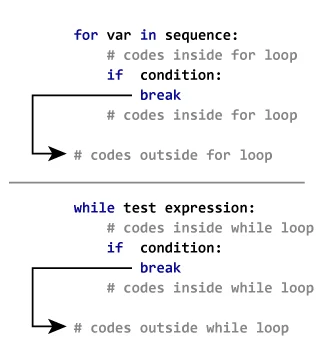
\includegraphics{./images/break.png}
  \caption{break}
  \end{figure}
\end{itemize}

    \begin{tcolorbox}[breakable, size=fbox, boxrule=1pt, pad at break*=1mm,colback=cellbackground, colframe=cellborder]
\prompt{In}{incolor}{25}{\boxspacing}
\begin{Verbatim}[commandchars=\\\{\}]
\PY{k}{for} \PY{n}{val} \PY{o+ow}{in} \PY{l+s+s2}{\PYZdq{}}\PY{l+s+s2}{string}\PY{l+s+s2}{\PYZdq{}}\PY{p}{:}
    \PY{k}{if} \PY{n}{val} \PY{o}{==} \PY{l+s+s2}{\PYZdq{}}\PY{l+s+s2}{i}\PY{l+s+s2}{\PYZdq{}}\PY{p}{:}
        \PY{k}{break}
    \PY{n+nb}{print}\PY{p}{(}\PY{n}{val}\PY{p}{)}

\PY{n+nb}{print}\PY{p}{(}\PY{l+s+s2}{\PYZdq{}}\PY{l+s+s2}{The end}\PY{l+s+s2}{\PYZdq{}}\PY{p}{)}
\end{Verbatim}
\end{tcolorbox}

    \begin{Verbatim}[commandchars=\\\{\}]
s
t
r
The end
    \end{Verbatim}

    \begin{itemize}
\item
  \texttt{continue} 的工作方式

  \begin{figure}
  \centering
  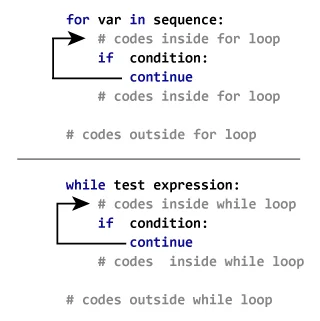
\includegraphics{./images/continue.png}
  \caption{continue}
  \end{figure}
\end{itemize}

    \begin{tcolorbox}[breakable, size=fbox, boxrule=1pt, pad at break*=1mm,colback=cellbackground, colframe=cellborder]
\prompt{In}{incolor}{26}{\boxspacing}
\begin{Verbatim}[commandchars=\\\{\}]
\PY{k}{for} \PY{n}{val} \PY{o+ow}{in} \PY{l+s+s2}{\PYZdq{}}\PY{l+s+s2}{string}\PY{l+s+s2}{\PYZdq{}}\PY{p}{:}
    \PY{k}{if} \PY{n}{val} \PY{o}{==} \PY{l+s+s2}{\PYZdq{}}\PY{l+s+s2}{i}\PY{l+s+s2}{\PYZdq{}}\PY{p}{:}
        \PY{k}{continue}
    \PY{n+nb}{print}\PY{p}{(}\PY{n}{val}\PY{p}{)}

\PY{n+nb}{print}\PY{p}{(}\PY{l+s+s2}{\PYZdq{}}\PY{l+s+s2}{The end}\PY{l+s+s2}{\PYZdq{}}\PY{p}{)}
\end{Verbatim}
\end{tcolorbox}

    \begin{Verbatim}[commandchars=\\\{\}]
s
t
r
n
g
The end
    \end{Verbatim}

    \begin{tcolorbox}[breakable, size=fbox, boxrule=1pt, pad at break*=1mm,colback=cellbackground, colframe=cellborder]
\prompt{In}{incolor}{27}{\boxspacing}
\begin{Verbatim}[commandchars=\\\{\}]
\PY{n}{a} \PY{o}{=} \PY{l+m+mi}{0}
\PY{k}{while} \PY{n}{a} \PY{o}{\PYZlt{}} \PY{l+m+mi}{30}\PY{p}{:}
    \PY{n+nb}{print}\PY{p}{(}\PY{n}{a}\PY{p}{)}
    \PY{k}{if} \PY{n}{a} \PY{o}{\PYZlt{}} \PY{l+m+mi}{3}\PY{p}{:}
        \PY{n}{a} \PY{o}{+}\PY{o}{=} \PY{l+m+mi}{1}
    \PY{k}{elif} \PY{n}{a} \PY{o}{\PYZlt{}} \PY{l+m+mi}{30}\PY{p}{:}
        \PY{n}{a} \PY{o}{+}\PY{o}{=} \PY{l+m+mi}{10}
    \PY{k}{else}\PY{p}{:}
        \PY{k}{break}
\PY{k}{else}\PY{p}{:}
    \PY{n+nb}{print}\PY{p}{(}\PY{l+s+s1}{\PYZsq{}}\PY{l+s+s1}{WoW}\PY{l+s+s1}{\PYZsq{}}\PY{p}{)}
\end{Verbatim}
\end{tcolorbox}

    \begin{Verbatim}[commandchars=\\\{\}]
0
1
2
3
13
23
WoW
    \end{Verbatim}

    \begin{itemize}
\tightlist
\item
  15. 布尔表达式的使用
\end{itemize}

    \begin{longtable}[]{@{}ll@{}}
\toprule
运算 & 含意 \\
\midrule
\endhead
\texttt{\textless{}} & 严格小于 \\
\texttt{\textless{}=} & 小于或等于 \\
\texttt{\textgreater{}} & 严格大于 \\
\texttt{\textgreater{}=} & 大于或等于 \\
\texttt{==} & 等于 \\
\texttt{!=} & 不等于 \\
\texttt{is} & 对象标识 \\
\texttt{is\ not} & 否定的对象标识 \\
\bottomrule
\end{longtable}

    \begin{longtable}[]{@{}ll@{}}
\toprule
运算 & 结果 \\
\midrule
\endhead
\texttt{x\ or\ y} & if x is false, then y, else x \\
\texttt{x\ and\ y} & if x is false, then x, else y \\
\texttt{not\ x} & if x is false, then True, else False \\
\bottomrule
\end{longtable}

    \begin{itemize}
\item
  16.
  循环语句中可迭代的结构:range、字符串、列表、元组、集合、字典、文件

  \begin{itemize}
  \item
    range 类型表示不可变的数字序列,通常用于在 for
    循环中循环指定的次数。

\begin{Shaded}
\begin{Highlighting}[]
\BuiltInTok{range}\NormalTok{(stop)}
\BuiltInTok{range}\NormalTok{(start, stop[, step])}
\end{Highlighting}
\end{Shaded}
  \end{itemize}
\end{itemize}

    \begin{tcolorbox}[breakable, size=fbox, boxrule=1pt, pad at break*=1mm,colback=cellbackground, colframe=cellborder]
\prompt{In}{incolor}{28}{\boxspacing}
\begin{Verbatim}[commandchars=\\\{\}]
\PY{n+nb}{print}\PY{p}{(}\PY{n+nb}{list}\PY{p}{(}\PY{n+nb}{range}\PY{p}{(}\PY{l+m+mi}{5}\PY{p}{)}\PY{p}{)}\PY{p}{)}
\PY{n+nb}{print}\PY{p}{(}\PY{n+nb}{list}\PY{p}{(}\PY{n+nb}{range}\PY{p}{(}\PY{l+m+mi}{1}\PY{p}{,} \PY{l+m+mi}{5}\PY{p}{)}\PY{p}{)}\PY{p}{)}
\PY{n+nb}{print}\PY{p}{(}\PY{n+nb}{list}\PY{p}{(}\PY{n+nb}{range}\PY{p}{(}\PY{l+m+mi}{0}\PY{p}{,} \PY{l+m+mi}{30}\PY{p}{,} \PY{l+m+mi}{5}\PY{p}{)}\PY{p}{)}\PY{p}{)}
\end{Verbatim}
\end{tcolorbox}

    \begin{Verbatim}[commandchars=\\\{\}]
[0, 1, 2, 3, 4]
[1, 2, 3, 4]
[0, 5, 10, 15, 20, 25]
    \end{Verbatim}

    \begin{tcolorbox}[breakable, size=fbox, boxrule=1pt, pad at break*=1mm,colback=cellbackground, colframe=cellborder]
\prompt{In}{incolor}{29}{\boxspacing}
\begin{Verbatim}[commandchars=\\\{\}]
\PY{k}{for} \PY{n}{n} \PY{o+ow}{in} \PY{n+nb}{range}\PY{p}{(}\PY{l+m+mi}{5}\PY{p}{)}\PY{p}{:}
    \PY{n+nb}{print}\PY{p}{(}\PY{n}{n}\PY{p}{,} \PY{n}{end}\PY{o}{=}\PY{l+s+s1}{\PYZsq{}}\PY{l+s+s1}{ }\PY{l+s+s1}{\PYZsq{}}\PY{p}{)}
\end{Verbatim}
\end{tcolorbox}

    \begin{Verbatim}[commandchars=\\\{\}]
0 1 2 3 4
    \end{Verbatim}

    \begin{tcolorbox}[breakable, size=fbox, boxrule=1pt, pad at break*=1mm,colback=cellbackground, colframe=cellborder]
\prompt{In}{incolor}{30}{\boxspacing}
\begin{Verbatim}[commandchars=\\\{\}]
\PY{k}{for} \PY{n}{c} \PY{o+ow}{in} \PY{l+s+s1}{\PYZsq{}}\PY{l+s+s1}{string}\PY{l+s+s1}{\PYZsq{}}\PY{p}{:}
    \PY{n+nb}{print}\PY{p}{(}\PY{n}{c}\PY{p}{,} \PY{n}{end} \PY{o}{=} \PY{l+s+s1}{\PYZsq{}}\PY{l+s+s1}{ }\PY{l+s+s1}{\PYZsq{}}\PY{p}{)}
\end{Verbatim}
\end{tcolorbox}

    \begin{Verbatim}[commandchars=\\\{\}]
s t r i n g
    \end{Verbatim}

    \begin{tcolorbox}[breakable, size=fbox, boxrule=1pt, pad at break*=1mm,colback=cellbackground, colframe=cellborder]
\prompt{In}{incolor}{31}{\boxspacing}
\begin{Verbatim}[commandchars=\\\{\}]
\PY{k}{for} \PY{n}{l} \PY{o+ow}{in} \PY{p}{[}\PY{l+s+s1}{\PYZsq{}}\PY{l+s+s1}{one}\PY{l+s+s1}{\PYZsq{}}\PY{p}{,} \PY{l+s+s1}{\PYZsq{}}\PY{l+s+s1}{two}\PY{l+s+s1}{\PYZsq{}}\PY{p}{,} \PY{l+s+s1}{\PYZsq{}}\PY{l+s+s1}{three}\PY{l+s+s1}{\PYZsq{}}\PY{p}{]}\PY{p}{:}
    \PY{n+nb}{print}\PY{p}{(}\PY{n}{l}\PY{p}{)}
\end{Verbatim}
\end{tcolorbox}

    \begin{Verbatim}[commandchars=\\\{\}]
one
two
three
    \end{Verbatim}

    \begin{tcolorbox}[breakable, size=fbox, boxrule=1pt, pad at break*=1mm,colback=cellbackground, colframe=cellborder]
\prompt{In}{incolor}{32}{\boxspacing}
\begin{Verbatim}[commandchars=\\\{\}]
\PY{k}{for} \PY{n}{k}\PY{p}{,} \PY{n}{v} \PY{o+ow}{in} \PY{p}{\PYZob{}}\PY{l+m+mi}{1}\PY{p}{:}\PY{l+s+s1}{\PYZsq{}}\PY{l+s+s1}{one}\PY{l+s+s1}{\PYZsq{}}\PY{p}{,} \PY{l+m+mi}{2}\PY{p}{:}\PY{l+s+s1}{\PYZsq{}}\PY{l+s+s1}{two}\PY{l+s+s1}{\PYZsq{}}\PY{p}{,} \PY{l+m+mi}{3}\PY{p}{:}\PY{l+s+s1}{\PYZsq{}}\PY{l+s+s1}{three}\PY{l+s+s1}{\PYZsq{}}\PY{p}{\PYZcb{}}\PY{o}{.}\PY{n}{items}\PY{p}{(}\PY{p}{)}\PY{p}{:}
    \PY{n+nb}{print}\PY{p}{(}\PY{n}{k}\PY{p}{,} \PY{n}{v}\PY{p}{)}
\end{Verbatim}
\end{tcolorbox}

    \begin{Verbatim}[commandchars=\\\{\}]
1 one
2 two
3 three
    \end{Verbatim}

    \begin{itemize}
\tightlist
\item
  17. 列表操作的方法

  \begin{itemize}
  \tightlist
  \item
    \texttt{append(x)} - 在列表末尾添加一个元素。
  \item
    \texttt{pop({[}i{]})} -
    删除列表中指定位置的元素,并返回被删除的元素。未指定位置时,a.pop()
    删除并返回列表的最后一个元素。
  \end{itemize}
\end{itemize}

    \begin{tcolorbox}[breakable, size=fbox, boxrule=1pt, pad at break*=1mm,colback=cellbackground, colframe=cellborder]
\prompt{In}{incolor}{33}{\boxspacing}
\begin{Verbatim}[commandchars=\\\{\}]
\PY{n}{fruits} \PY{o}{=} \PY{p}{[}\PY{l+s+s1}{\PYZsq{}}\PY{l+s+s1}{orange}\PY{l+s+s1}{\PYZsq{}}\PY{p}{,} \PY{l+s+s1}{\PYZsq{}}\PY{l+s+s1}{apple}\PY{l+s+s1}{\PYZsq{}}\PY{p}{,} \PY{l+s+s1}{\PYZsq{}}\PY{l+s+s1}{pear}\PY{l+s+s1}{\PYZsq{}}\PY{p}{,} \PY{l+s+s1}{\PYZsq{}}\PY{l+s+s1}{banana}\PY{l+s+s1}{\PYZsq{}}\PY{p}{,} \PY{l+s+s1}{\PYZsq{}}\PY{l+s+s1}{kiwi}\PY{l+s+s1}{\PYZsq{}}\PY{p}{,} \PY{l+s+s1}{\PYZsq{}}\PY{l+s+s1}{apple}\PY{l+s+s1}{\PYZsq{}}\PY{p}{,} \PY{l+s+s1}{\PYZsq{}}\PY{l+s+s1}{banana}\PY{l+s+s1}{\PYZsq{}}\PY{p}{]}
\PY{n+nb}{print}\PY{p}{(}\PY{n}{fruits}\PY{p}{)}
\PY{n}{fruits}\PY{o}{.}\PY{n}{append}\PY{p}{(}\PY{l+s+s1}{\PYZsq{}}\PY{l+s+s1}{mongo}\PY{l+s+s1}{\PYZsq{}}\PY{p}{)}  \PY{c+c1}{\PYZsh{} 追加一个元素}
\PY{n+nb}{print}\PY{p}{(}\PY{n}{fruits}\PY{p}{)}
\PY{n}{fruits}\PY{o}{.}\PY{n}{pop}\PY{p}{(}\PY{l+m+mi}{3}\PY{p}{)}  \PY{c+c1}{\PYZsh{} 删除第五个元素 banana}
\PY{n}{fruits}\PY{o}{.}\PY{n}{pop}\PY{p}{(}\PY{l+m+mi}{3}\PY{p}{)}  \PY{c+c1}{\PYZsh{} 删除第五个元素 kiwi}
\PY{n+nb}{print}\PY{p}{(}\PY{n}{fruits}\PY{p}{)}
\PY{n}{fruits}\PY{o}{.}\PY{n}{pop}\PY{p}{(}\PY{p}{)}   \PY{c+c1}{\PYZsh{} 删除最后一个元素 mongo}
\PY{n+nb}{print}\PY{p}{(}\PY{n}{fruits}\PY{p}{)}
\end{Verbatim}
\end{tcolorbox}

    \begin{Verbatim}[commandchars=\\\{\}]
['orange', 'apple', 'pear', 'banana', 'kiwi', 'apple', 'banana']
['orange', 'apple', 'pear', 'banana', 'kiwi', 'apple', 'banana', 'mongo']
['orange', 'apple', 'pear', 'apple', 'banana', 'mongo']
['orange', 'apple', 'pear', 'apple', 'banana']
    \end{Verbatim}

    \begin{itemize}
\tightlist
\item
  18.
  列表的排序方法\texttt{sort()}以及内置函数\texttt{sorted()}的应用场合、语法、排序规则的指定(lambda函数)、返回值等
\end{itemize}

    \begin{tcolorbox}[breakable, size=fbox, boxrule=1pt, pad at break*=1mm,colback=cellbackground, colframe=cellborder]
\prompt{In}{incolor}{34}{\boxspacing}
\begin{Verbatim}[commandchars=\\\{\}]
\PY{c+c1}{\PYZsh{} TODO}
\end{Verbatim}
\end{tcolorbox}

    \begin{itemize}
\tightlist
\item
  19. 元组的非正规写法

  \begin{itemize}
  \tightlist
  \item
    多变量赋值
  \item
    两变量值交换
  \end{itemize}
\end{itemize}

    \begin{tcolorbox}[breakable, size=fbox, boxrule=1pt, pad at break*=1mm,colback=cellbackground, colframe=cellborder]
\prompt{In}{incolor}{35}{\boxspacing}
\begin{Verbatim}[commandchars=\\\{\}]
\PY{c+c1}{\PYZsh{} 多变量赋值}
\PY{n}{a}\PY{p}{,} \PY{n}{b}\PY{p}{,} \PY{p}{(}\PY{n}{c}\PY{p}{,} \PY{n}{d}\PY{p}{)}\PY{p}{,} \PY{n}{e} \PY{o}{=} \PY{l+m+mi}{1}\PY{p}{,} \PY{l+m+mi}{3}\PY{p}{,} \PY{p}{(}\PY{l+m+mi}{5}\PY{p}{,} \PY{l+m+mi}{7}\PY{p}{)}\PY{p}{,} \PY{l+m+mi}{9}
\PY{n+nb}{print}\PY{p}{(}\PY{n}{a}\PY{p}{,} \PY{n}{b}\PY{p}{,} \PY{n}{c}\PY{p}{,} \PY{n}{d}\PY{p}{,} \PY{n}{e}\PY{p}{,} \PY{n}{sep} \PY{o}{=} \PY{l+s+s1}{\PYZsq{}}\PY{l+s+s1}{, }\PY{l+s+s1}{\PYZsq{}}\PY{p}{)}

\PY{c+c1}{\PYZsh{} 两变量值交换}
\PY{n}{x}\PY{p}{,} \PY{n}{y} \PY{o}{=} \PY{l+s+s1}{\PYZsq{}}\PY{l+s+s1}{hello}\PY{l+s+s1}{\PYZsq{}}\PY{p}{,} \PY{l+s+s1}{\PYZsq{}}\PY{l+s+s1}{world}\PY{l+s+s1}{\PYZsq{}}
\PY{n}{x}\PY{p}{,} \PY{n}{y} \PY{o}{=} \PY{n}{y}\PY{p}{,} \PY{n}{x}
\PY{n+nb}{print}\PY{p}{(}\PY{n}{x}\PY{p}{,} \PY{n}{y}\PY{p}{)}
\end{Verbatim}
\end{tcolorbox}

    \begin{Verbatim}[commandchars=\\\{\}]
1, 3, 5, 7, 9
world hello
    \end{Verbatim}

    \begin{itemize}
\tightlist
\item
  20. 元组的基本要求和操作

  \begin{itemize}
  \tightlist
  \item
    利用列表里面嵌套元组完成相应应用描述,并能进行操作
  \end{itemize}
\item
  21. 集合运算符:\texttt{\&}, \texttt{\textbar{}},
  \texttt{-}(只要求能读懂程序)
\end{itemize}

    \begin{tcolorbox}[breakable, size=fbox, boxrule=1pt, pad at break*=1mm,colback=cellbackground, colframe=cellborder]
\prompt{In}{incolor}{36}{\boxspacing}
\begin{Verbatim}[commandchars=\\\{\}]
\PY{n}{girls} \PY{o}{=} \PY{p}{\PYZob{}}\PY{l+s+s1}{\PYZsq{}}\PY{l+s+s1}{Adele}\PY{l+s+s1}{\PYZsq{}}\PY{p}{,} \PY{l+s+s1}{\PYZsq{}}\PY{l+s+s1}{Lady Gaga}\PY{l+s+s1}{\PYZsq{}}\PY{p}{,} \PY{l+s+s1}{\PYZsq{}}\PY{l+s+s1}{G.E.M}\PY{l+s+s1}{\PYZsq{}}\PY{p}{\PYZcb{}}
\PY{n}{boys} \PY{o}{=} \PY{p}{\PYZob{}}\PY{l+s+s1}{\PYZsq{}}\PY{l+s+s1}{Jay Zhou}\PY{l+s+s1}{\PYZsq{}}\PY{p}{,} \PY{l+s+s1}{\PYZsq{}}\PY{l+s+s1}{Ed Sheeran}\PY{l+s+s1}{\PYZsq{}}\PY{p}{,} \PY{l+s+s1}{\PYZsq{}}\PY{l+s+s1}{Justin Bieber}\PY{l+s+s1}{\PYZsq{}}\PY{p}{\PYZcb{}}
\PY{n}{chinese} \PY{o}{=} \PY{p}{\PYZob{}}\PY{l+s+s1}{\PYZsq{}}\PY{l+s+s1}{G.E.M}\PY{l+s+s1}{\PYZsq{}}\PY{p}{,} \PY{l+s+s1}{\PYZsq{}}\PY{l+s+s1}{Jay Zhou}\PY{l+s+s1}{\PYZsq{}}\PY{p}{\PYZcb{}}
\PY{n}{singers} \PY{o}{=} \PY{n}{girls} \PY{o}{|} \PY{n}{boys}
\PY{n}{chineseBoys} \PY{o}{=} \PY{n}{chinese} \PY{o}{\PYZam{}} \PY{n}{boys}
\PY{n}{foreignGirls} \PY{o}{=} \PY{n}{girls} \PY{o}{\PYZhy{}} \PY{n}{chinese}
\PY{n+nb}{print}\PY{p}{(}\PY{n}{singers}\PY{p}{,} \PY{n}{chineseBoys}\PY{p}{,} \PY{n}{foreignGirls}\PY{p}{,} \PY{n}{sep} \PY{o}{=} \PY{l+s+s1}{\PYZsq{}}\PY{l+s+se}{\PYZbs{}n}\PY{l+s+s1}{\PYZsq{}}\PY{p}{)}
\end{Verbatim}
\end{tcolorbox}

    \begin{Verbatim}[commandchars=\\\{\}]
\{'Lady Gaga', 'G.E.M', 'Jay Zhou', 'Justin Bieber', 'Adele', 'Ed Sheeran'\}
\{'Jay Zhou'\}
\{'Lady Gaga', 'Adele'\}
    \end{Verbatim}

    \begin{itemize}
\tightlist
\item
  22. 集合操作的方法:\texttt{add()}
\end{itemize}

    \begin{tcolorbox}[breakable, size=fbox, boxrule=1pt, pad at break*=1mm,colback=cellbackground, colframe=cellborder]
\prompt{In}{incolor}{37}{\boxspacing}
\begin{Verbatim}[commandchars=\\\{\}]
\PY{n}{girls} \PY{o}{=} \PY{p}{\PYZob{}}\PY{l+s+s1}{\PYZsq{}}\PY{l+s+s1}{Adele}\PY{l+s+s1}{\PYZsq{}}\PY{p}{,} \PY{l+s+s1}{\PYZsq{}}\PY{l+s+s1}{Lady Gaga}\PY{l+s+s1}{\PYZsq{}}\PY{p}{,} \PY{l+s+s1}{\PYZsq{}}\PY{l+s+s1}{G.E.M}\PY{l+s+s1}{\PYZsq{}}\PY{p}{\PYZcb{}}
\PY{n}{girls}\PY{o}{.}\PY{n}{add}\PY{p}{(}\PY{l+s+s1}{\PYZsq{}}\PY{l+s+s1}{WanTing}\PY{l+s+s1}{\PYZsq{}}\PY{p}{)}
\PY{n+nb}{print}\PY{p}{(}\PY{n}{girls}\PY{p}{)}
\end{Verbatim}
\end{tcolorbox}

    \begin{Verbatim}[commandchars=\\\{\}]
\{'Lady Gaga', 'WanTing', 'Adele', 'G.E.M'\}
    \end{Verbatim}

    \begin{itemize}
\tightlist
\item
  23. 集合的去除重复工作
\end{itemize}

    \begin{tcolorbox}[breakable, size=fbox, boxrule=1pt, pad at break*=1mm,colback=cellbackground, colframe=cellborder]
\prompt{In}{incolor}{38}{\boxspacing}
\begin{Verbatim}[commandchars=\\\{\}]
\PY{n}{l} \PY{o}{=} \PY{n+nb}{list}\PY{p}{(}\PY{l+s+s1}{\PYZsq{}}\PY{l+s+s1}{Hello world, my girl!}\PY{l+s+s1}{\PYZsq{}}\PY{p}{)}

\PY{c+c1}{\PYZsh{} 顺序无关}
\PY{n}{unique} \PY{o}{=} \PY{n+nb}{list}\PY{p}{(}\PY{n+nb}{set}\PY{p}{(}\PY{n}{l}\PY{p}{)}\PY{p}{)}
\PY{n+nb}{print}\PY{p}{(}\PY{n}{unique}\PY{p}{)}

\PY{c+c1}{\PYZsh{} 顺序有关}
\PY{n}{unique} \PY{o}{=} \PY{p}{[}\PY{p}{]}
\PY{n}{seen} \PY{o}{=} \PY{n+nb}{set}\PY{p}{(}\PY{p}{)}
\PY{k}{for} \PY{n}{e} \PY{o+ow}{in} \PY{n}{l}\PY{p}{:}
    \PY{k}{if} \PY{n}{e} \PY{o+ow}{in} \PY{n}{seen}\PY{p}{:}
        \PY{k}{continue}
    \PY{k}{else}\PY{p}{:}
        \PY{n}{unique}\PY{o}{.}\PY{n}{append}\PY{p}{(}\PY{n}{e}\PY{p}{)}
        \PY{n}{seen}\PY{o}{.}\PY{n}{add}\PY{p}{(}\PY{n}{e}\PY{p}{)}
\PY{n+nb}{print}\PY{p}{(}\PY{n}{unique}\PY{p}{)}
\end{Verbatim}
\end{tcolorbox}

    \begin{Verbatim}[commandchars=\\\{\}]
['y', 'd', 'm', 'g', 'l', ',', 'w', 'H', 'i', 'r', ' ', '!', 'e', 'o']
['H', 'e', 'l', 'o', ' ', 'w', 'r', 'd', ',', 'm', 'y', 'g', 'i', '!']
    \end{Verbatim}

    \begin{itemize}
\tightlist
\item
  24. 字典添加新的键值对
\end{itemize}

    \begin{tcolorbox}[breakable, size=fbox, boxrule=1pt, pad at break*=1mm,colback=cellbackground, colframe=cellborder]
\prompt{In}{incolor}{39}{\boxspacing}
\begin{Verbatim}[commandchars=\\\{\}]
\PY{n}{d} \PY{o}{=} \PY{p}{\PYZob{}}\PY{l+s+s1}{\PYZsq{}}\PY{l+s+s1}{whale}\PY{l+s+s1}{\PYZsq{}}\PY{p}{:} \PY{l+m+mi}{5}\PY{p}{,} \PY{l+s+s1}{\PYZsq{}}\PY{l+s+s1}{shark}\PY{l+s+s1}{\PYZsq{}}\PY{p}{:} \PY{l+m+mi}{3}\PY{p}{\PYZcb{}}
\PY{n+nb}{print}\PY{p}{(}\PY{n}{d}\PY{p}{)}
\PY{n}{d}\PY{p}{[}\PY{l+s+s1}{\PYZsq{}}\PY{l+s+s1}{python}\PY{l+s+s1}{\PYZsq{}}\PY{p}{]} \PY{o}{=} \PY{l+m+mi}{9} \PY{c+c1}{\PYZsh{} Add 1}
\PY{n+nb}{print}\PY{p}{(}\PY{n}{d}\PY{p}{)}
\PY{n}{d}\PY{o}{.}\PY{n}{update}\PY{p}{(}\PY{p}{\PYZob{}}\PY{l+s+s1}{\PYZsq{}}\PY{l+s+s1}{shrimp}\PY{l+s+s1}{\PYZsq{}}\PY{p}{:} \PY{l+m+mi}{10000}\PY{p}{,} \PY{l+s+s1}{\PYZsq{}}\PY{l+s+s1}{kraken}\PY{l+s+s1}{\PYZsq{}}\PY{p}{:} \PY{l+m+mi}{1}\PY{p}{,} \PY{l+s+s1}{\PYZsq{}}\PY{l+s+s1}{serpant}\PY{l+s+s1}{\PYZsq{}}\PY{p}{:} \PY{l+m+mi}{2}\PY{p}{\PYZcb{}}\PY{p}{)} \PY{c+c1}{\PYZsh{} Add many}
\PY{n+nb}{print}\PY{p}{(}\PY{n}{d}\PY{p}{)}
\end{Verbatim}
\end{tcolorbox}

    \begin{Verbatim}[commandchars=\\\{\}]
\{'whale': 5, 'shark': 3\}
\{'whale': 5, 'shark': 3, 'python': 9\}
\{'whale': 5, 'shark': 3, 'python': 9, 'shrimp': 10000, 'kraken': 1, 'serpant':
2\}
    \end{Verbatim}

    \begin{itemize}
\tightlist
\item
  25. 字典中键、值、键值对的获取 \texttt{keys()}, \texttt{values()},
  \texttt{items()}

  \begin{itemize}
  \tightlist
  \item
    对字典元素的迭代默认情况是对键的迭代
  \item
    能够用字典描述特定键值对类型的应用并操作
  \end{itemize}
\end{itemize}

    \begin{tcolorbox}[breakable, size=fbox, boxrule=1pt, pad at break*=1mm,colback=cellbackground, colframe=cellborder]
\prompt{In}{incolor}{40}{\boxspacing}
\begin{Verbatim}[commandchars=\\\{\}]
\PY{n}{d} \PY{o}{=} \PY{p}{\PYZob{}}\PY{l+s+s1}{\PYZsq{}}\PY{l+s+s1}{whale}\PY{l+s+s1}{\PYZsq{}}\PY{p}{:} \PY{l+m+mi}{5}\PY{p}{,} \PY{l+s+s1}{\PYZsq{}}\PY{l+s+s1}{shark}\PY{l+s+s1}{\PYZsq{}}\PY{p}{:} \PY{l+m+mi}{3}\PY{p}{,} \PY{l+s+s1}{\PYZsq{}}\PY{l+s+s1}{python}\PY{l+s+s1}{\PYZsq{}}\PY{p}{:} \PY{l+m+mi}{19}\PY{p}{\PYZcb{}}
\PY{n+nb}{print}\PY{p}{(}\PY{n}{d}\PY{o}{.}\PY{n}{keys}\PY{p}{(}\PY{p}{)}\PY{p}{)}
\PY{n+nb}{print}\PY{p}{(}\PY{n}{d}\PY{o}{.}\PY{n}{values}\PY{p}{(}\PY{p}{)}\PY{p}{)}
\PY{n+nb}{print}\PY{p}{(}\PY{n}{d}\PY{o}{.}\PY{n}{items}\PY{p}{(}\PY{p}{)}\PY{p}{)}
\PY{k}{for} \PY{n}{k} \PY{o+ow}{in} \PY{n}{d}\PY{p}{:}
    \PY{n+nb}{print}\PY{p}{(}\PY{n}{k}\PY{p}{)}
\PY{k}{for} \PY{n}{k}\PY{p}{,} \PY{n}{v} \PY{o+ow}{in} \PY{n}{d}\PY{o}{.}\PY{n}{items}\PY{p}{(}\PY{p}{)}\PY{p}{:}
    \PY{n+nb}{print}\PY{p}{(}\PY{l+s+s1}{\PYZsq{}}\PY{l+s+s1}{the number of }\PY{l+s+si}{\PYZob{}:\PYZlt{}6\PYZcb{}}\PY{l+s+s1}{ = }\PY{l+s+si}{\PYZob{}:\PYZgt{}2\PYZcb{}}\PY{l+s+s1}{\PYZsq{}}\PY{o}{.}\PY{n}{format}\PY{p}{(}\PY{n}{k}\PY{p}{,} \PY{n}{v}\PY{p}{)}\PY{p}{)}
\end{Verbatim}
\end{tcolorbox}

    \begin{Verbatim}[commandchars=\\\{\}]
dict\_keys(['whale', 'shark', 'python'])
dict\_values([5, 3, 19])
dict\_items([('whale', 5), ('shark', 3), ('python', 19)])
whale
shark
python
the number of whale  =  5
the number of shark  =  3
the number of python = 19
    \end{Verbatim}

    \begin{itemize}
\item
  26. 字典的\texttt{get()}方法的作用及使用

  \texttt{get(key{[},\ default{]})} \textgreater{} 如果 key
  存在于字典中则返回 key 的值,否则返回 default。 如果 default
  未给出则默认为 None,因而此方法绝不会引发 KeyError。
\end{itemize}

    \begin{tcolorbox}[breakable, size=fbox, boxrule=1pt, pad at break*=1mm,colback=cellbackground, colframe=cellborder]
\prompt{In}{incolor}{41}{\boxspacing}
\begin{Verbatim}[commandchars=\\\{\}]
\PY{n}{d} \PY{o}{=} \PY{p}{\PYZob{}}\PY{l+s+s1}{\PYZsq{}}\PY{l+s+s1}{whale}\PY{l+s+s1}{\PYZsq{}}\PY{p}{:} \PY{l+m+mi}{5}\PY{p}{,} \PY{l+s+s1}{\PYZsq{}}\PY{l+s+s1}{shark}\PY{l+s+s1}{\PYZsq{}}\PY{p}{:} \PY{l+m+mi}{3}\PY{p}{,} \PY{l+s+s1}{\PYZsq{}}\PY{l+s+s1}{python}\PY{l+s+s1}{\PYZsq{}}\PY{p}{:} \PY{l+m+mi}{19}\PY{p}{\PYZcb{}}
\PY{n+nb}{print}\PY{p}{(}\PY{n}{d}\PY{p}{[}\PY{l+s+s1}{\PYZsq{}}\PY{l+s+s1}{whale}\PY{l+s+s1}{\PYZsq{}}\PY{p}{]}\PY{p}{)}
\PY{c+c1}{\PYZsh{} print(d[\PYZsq{}shrimp\PYZsq{}])         \PYZsh{} shrimp 不存在,报错}
\PY{n+nb}{print}\PY{p}{(}\PY{n}{d}\PY{o}{.}\PY{n}{get}\PY{p}{(}\PY{l+s+s1}{\PYZsq{}}\PY{l+s+s1}{whale}\PY{l+s+s1}{\PYZsq{}}\PY{p}{)}\PY{p}{)}
\PY{n+nb}{print}\PY{p}{(}\PY{n}{d}\PY{o}{.}\PY{n}{get}\PY{p}{(}\PY{l+s+s1}{\PYZsq{}}\PY{l+s+s1}{shrimp}\PY{l+s+s1}{\PYZsq{}}\PY{p}{)}\PY{p}{)}       \PY{c+c1}{\PYZsh{} shrimp 不存在,不报错}
\PY{n+nb}{print}\PY{p}{(}\PY{n}{d}\PY{o}{.}\PY{n}{get}\PY{p}{(}\PY{l+s+s1}{\PYZsq{}}\PY{l+s+s1}{shrimp}\PY{l+s+s1}{\PYZsq{}}\PY{p}{,} \PY{l+m+mi}{999}\PY{p}{)}\PY{p}{)}  \PY{c+c1}{\PYZsh{} shrimp 不存在,返回默认值}
\end{Verbatim}
\end{tcolorbox}

    \begin{Verbatim}[commandchars=\\\{\}]
5
5
None
999
    \end{Verbatim}

    \begin{itemize}
\tightlist
\item
  27. 函数定义及简单参数传递
\end{itemize}

    \begin{tcolorbox}[breakable, size=fbox, boxrule=1pt, pad at break*=1mm,colback=cellbackground, colframe=cellborder]
\prompt{In}{incolor}{42}{\boxspacing}
\begin{Verbatim}[commandchars=\\\{\}]
\PY{c+c1}{\PYZsh{} TODO}
\end{Verbatim}
\end{tcolorbox}

    \begin{itemize}
\tightlist
\item
  28.
  使用pip工具查看当前已安装的Python扩展库的完整命令\texttt{pip\ list},安装扩展库命令\texttt{pip\ install}库名。

  \begin{itemize}
  \item
    pip list

\begin{Shaded}
\begin{Highlighting}[]
\NormalTok{$ pip list}
\NormalTok{Package              Version}
\NormalTok{{-}{-}{-}{-}{-}{-}{-}{-}{-}{-}{-}{-}{-}{-}{-}{-}{-}{-}{-}{-} {-}{-}{-}{-}{-}{-}{-}{-}{-}}
\NormalTok{appdirs              1.4.4}
\NormalTok{appnope              0.1.2}
\NormalTok{argon2{-}cffi          21.3.0}
\NormalTok{argon2{-}cffi{-}bindings 21.2.0}
\NormalTok{attrs                21.2.0}
\NormalTok{...}
\NormalTok{...}
\end{Highlighting}
\end{Shaded}
  \item
    pip install

\begin{Shaded}
\begin{Highlighting}[]
\NormalTok{$ pip install pandas}
\NormalTok{$ pip install wordcloud}
\NormalTok{$ pip install jieba}
\end{Highlighting}
\end{Shaded}
  \end{itemize}
\end{itemize}

    \begin{itemize}
\tightlist
\item
  29. 文件打开模式:\texttt{r}, \texttt{w}
\item
  30. 读文本文件的方法:\texttt{read()}, \texttt{readlines()}

  \begin{itemize}
  \tightlist
  \item
    对文件对象的迭代默认情况是\texttt{readlines()}
  \end{itemize}
\item
  31. 写文本文件的方法:\texttt{writelines()}
\item
  32. CSV库,json库读写文件操作的基本语法
\item
  33. 上下文管理器的应用:\texttt{with\ open()\ as\ f:}
\end{itemize}

    \begin{itemize}
\tightlist
\item
  34. 第三方库random的方法:\texttt{randint()}
\end{itemize}

    \begin{tcolorbox}[breakable, size=fbox, boxrule=1pt, pad at break*=1mm,colback=cellbackground, colframe=cellborder]
\prompt{In}{incolor}{43}{\boxspacing}
\begin{Verbatim}[commandchars=\\\{\}]
\PY{k+kn}{import} \PY{n+nn}{random}
\PY{n}{random}\PY{o}{.}\PY{n}{seed}\PY{p}{(}\PY{l+m+mi}{5}\PY{p}{)}
\PY{n}{x} \PY{o}{=} \PY{n}{random}\PY{o}{.}\PY{n}{randint}\PY{p}{(}\PY{l+m+mi}{0}\PY{p}{,} \PY{l+m+mi}{9}\PY{p}{)}  \PY{c+c1}{\PYZsh{} 唯一的闭区间[0, 9]}
\PY{n}{random}\PY{o}{.}\PY{n}{seed}\PY{p}{(}\PY{l+m+mi}{5}\PY{p}{)}        \PY{c+c1}{\PYZsh{} 同样的seed}
\PY{n}{y} \PY{o}{=} \PY{n}{random}\PY{o}{.}\PY{n}{randint}\PY{p}{(}\PY{l+m+mi}{0}\PY{p}{,} \PY{l+m+mi}{9}\PY{p}{)}  \PY{c+c1}{\PYZsh{} 得到同样的随机数}
\PY{n+nb}{print}\PY{p}{(}\PY{n}{x}\PY{p}{,} \PY{n}{y}\PY{p}{)}
\end{Verbatim}
\end{tcolorbox}

    \begin{Verbatim}[commandchars=\\\{\}]
9 9
    \end{Verbatim}

    \begin{tcolorbox}[breakable, size=fbox, boxrule=1pt, pad at break*=1mm,colback=cellbackground, colframe=cellborder]
\prompt{In}{incolor}{44}{\boxspacing}
\begin{Verbatim}[commandchars=\\\{\}]
\PY{k+kn}{import} \PY{n+nn}{random}
\PY{n}{cards} \PY{o}{=} \PY{n+nb}{list}\PY{p}{(}\PY{l+s+s1}{\PYZsq{}}\PY{l+s+s1}{A23456789JQK}\PY{l+s+s1}{\PYZsq{}}\PY{p}{)}
\PY{n}{random}\PY{o}{.}\PY{n}{shuffle}\PY{p}{(}\PY{n}{cards}\PY{p}{)}
\PY{n+nb}{print}\PY{p}{(}\PY{n}{cards}\PY{p}{)}
\PY{n}{random}\PY{o}{.}\PY{n}{shuffle}\PY{p}{(}\PY{n}{cards}\PY{p}{)}
\PY{n+nb}{print}\PY{p}{(}\PY{n}{cards}\PY{p}{)}
\end{Verbatim}
\end{tcolorbox}

    \begin{Verbatim}[commandchars=\\\{\}]
['3', '4', 'K', 'Q', 'J', '2', '7', '8', 'A', '9', '6', '5']
['9', 'K', '6', '2', '3', '5', 'J', '4', 'A', '7', 'Q', '8']
    \end{Verbatim}

    \begin{itemize}
\tightlist
\item
  35. 可视化:绘制饼图、直方图、多种折线图、散点图
\end{itemize}

    \begin{tcolorbox}[breakable, size=fbox, boxrule=1pt, pad at break*=1mm,colback=cellbackground, colframe=cellborder]
\prompt{In}{incolor}{45}{\boxspacing}
\begin{Verbatim}[commandchars=\\\{\}]
\PY{c+c1}{\PYZsh{} TODO}
\end{Verbatim}
\end{tcolorbox}

    \hypertarget{ux9898ux578b}{%
\subsection{题型}\label{ux9898ux578b}}

所有选择题和判断题均出自砺儒云平台的课前、课后测试题,只有个别题目做了适当修改

\begin{longtable}[]{@{}lll@{}}
\toprule
\# & 题型 & 分数 \\
\midrule
\endhead
1 & 选择题 & 10x2 \\
2 & 判断题 & 15x1 \\
3 & 程序分析题 & 5x5 \\
4 & 应用题(程序填空) & 10x2 \\
5 & 思维提升题(问答题) & 2x5 \\
6 & 应用创新题(编程题) & 1x10 \\
\bottomrule
\end{longtable}


    % Add a bibliography block to the postdoc
    
    
    
\end{document}
